% Options for packages loaded elsewhere
% !TEX program = xelatex
% Bản LaTeX được sinh từ seminar-detailed-report.md bằng Pandoc.
\PassOptionsToPackage{unicode}{hyperref}
\PassOptionsToPackage{hyphens}{url}
\PassOptionsToPackage{dvipsnames,svgnames,x11names}{xcolor}
\documentclass[
  vietnamese,
  12pt,
  a4paper,
  oneside]{report}
\usepackage{xcolor}
\usepackage[top=2.5cm,bottom=2.5cm,left=3cm,right=2cm]{geometry}
\usepackage{amsmath,amssymb}
\setcounter{secnumdepth}{-\maxdimen} % remove section numbering
\usepackage{iftex}
\ifPDFTeX
  \usepackage[T1]{fontenc}
  \usepackage[utf8]{inputenc}
  \usepackage{textcomp} % provide euro and other symbols
\else % if luatex or xetex
  \usepackage{unicode-math} % this also loads fontspec
  \defaultfontfeatures{Scale=MatchLowercase}
  \defaultfontfeatures[\rmfamily]{Ligatures=TeX,Scale=1}
\fi
\usepackage{lmodern}
\ifPDFTeX\else
  % xetex/luatex font selection
  \setmainfont[]{Times New Roman}
  \setsansfont[]{Arial}
  \setmonofont[]{Consolas}
\fi
% Use upquote if available, for straight quotes in verbatim environments
\IfFileExists{upquote.sty}{\usepackage{upquote}}{}
\IfFileExists{microtype.sty}{% use microtype if available
  \usepackage[]{microtype}
  \UseMicrotypeSet[protrusion]{basicmath} % disable protrusion for tt fonts
}{}
\usepackage{setspace}
\makeatletter
\@ifundefined{KOMAClassName}{% if non-KOMA class
  \IfFileExists{parskip.sty}{%
    \usepackage{parskip}
  }{% else
    \setlength{\parindent}{0pt}
    \setlength{\parskip}{6pt plus 2pt minus 1pt}}
}{% if KOMA class
  \KOMAoptions{parskip=half}}
\makeatother
\usepackage{color}
\usepackage{fancyvrb}
\newcommand{\VerbBar}{|}
\newcommand{\VERB}{\Verb[commandchars=\\\{\}]}
\DefineVerbatimEnvironment{Highlighting}{Verbatim}{commandchars=\\\{\}}
% Add ',fontsize=\small' for more characters per line
\newenvironment{Shaded}{}{}
\newcommand{\AlertTok}[1]{\textcolor[rgb]{1.00,0.00,0.00}{\textbf{#1}}}
\newcommand{\AnnotationTok}[1]{\textcolor[rgb]{0.38,0.63,0.69}{\textbf{\textit{#1}}}}
\newcommand{\AttributeTok}[1]{\textcolor[rgb]{0.49,0.56,0.16}{#1}}
\newcommand{\BaseNTok}[1]{\textcolor[rgb]{0.25,0.63,0.44}{#1}}
\newcommand{\BuiltInTok}[1]{\textcolor[rgb]{0.00,0.50,0.00}{#1}}
\newcommand{\CharTok}[1]{\textcolor[rgb]{0.25,0.44,0.63}{#1}}
\newcommand{\CommentTok}[1]{\textcolor[rgb]{0.38,0.63,0.69}{\textit{#1}}}
\newcommand{\CommentVarTok}[1]{\textcolor[rgb]{0.38,0.63,0.69}{\textbf{\textit{#1}}}}
\newcommand{\ConstantTok}[1]{\textcolor[rgb]{0.53,0.00,0.00}{#1}}
\newcommand{\ControlFlowTok}[1]{\textcolor[rgb]{0.00,0.44,0.13}{\textbf{#1}}}
\newcommand{\DataTypeTok}[1]{\textcolor[rgb]{0.56,0.13,0.00}{#1}}
\newcommand{\DecValTok}[1]{\textcolor[rgb]{0.25,0.63,0.44}{#1}}
\newcommand{\DocumentationTok}[1]{\textcolor[rgb]{0.73,0.13,0.13}{\textit{#1}}}
\newcommand{\ErrorTok}[1]{\textcolor[rgb]{1.00,0.00,0.00}{\textbf{#1}}}
\newcommand{\ExtensionTok}[1]{#1}
\newcommand{\FloatTok}[1]{\textcolor[rgb]{0.25,0.63,0.44}{#1}}
\newcommand{\FunctionTok}[1]{\textcolor[rgb]{0.02,0.16,0.49}{#1}}
\newcommand{\ImportTok}[1]{\textcolor[rgb]{0.00,0.50,0.00}{\textbf{#1}}}
\newcommand{\InformationTok}[1]{\textcolor[rgb]{0.38,0.63,0.69}{\textbf{\textit{#1}}}}
\newcommand{\KeywordTok}[1]{\textcolor[rgb]{0.00,0.44,0.13}{\textbf{#1}}}
\newcommand{\NormalTok}[1]{#1}
\newcommand{\OperatorTok}[1]{\textcolor[rgb]{0.40,0.40,0.40}{#1}}
\newcommand{\OtherTok}[1]{\textcolor[rgb]{0.00,0.44,0.13}{#1}}
\newcommand{\PreprocessorTok}[1]{\textcolor[rgb]{0.74,0.48,0.00}{#1}}
\newcommand{\RegionMarkerTok}[1]{#1}
\newcommand{\SpecialCharTok}[1]{\textcolor[rgb]{0.25,0.44,0.63}{#1}}
\newcommand{\SpecialStringTok}[1]{\textcolor[rgb]{0.73,0.40,0.53}{#1}}
\newcommand{\StringTok}[1]{\textcolor[rgb]{0.25,0.44,0.63}{#1}}
\newcommand{\VariableTok}[1]{\textcolor[rgb]{0.10,0.09,0.49}{#1}}
\newcommand{\VerbatimStringTok}[1]{\textcolor[rgb]{0.25,0.44,0.63}{#1}}
\newcommand{\WarningTok}[1]{\textcolor[rgb]{0.38,0.63,0.69}{\textbf{\textit{#1}}}}
\usepackage{longtable,booktabs,array}
\usepackage{calc} % for calculating minipage widths
% Correct order of tables after \paragraph or \subparagraph
\usepackage{etoolbox}
\makeatletter
\patchcmd\longtable{\par}{\if@noskipsec\mbox{}\fi\par}{}{}
\makeatother
% Allow footnotes in longtable head/foot
\IfFileExists{footnotehyper.sty}{\usepackage{footnotehyper}}{\usepackage{footnote}}
\makesavenoteenv{longtable}
\usepackage{graphicx}
\makeatletter
\newsavebox\pandoc@box
\newcommand*\pandocbounded[1]{% scales image to fit in text height/width
  \sbox\pandoc@box{#1}%
  \Gscale@div\@tempa{\textheight}{\dimexpr\ht\pandoc@box+\dp\pandoc@box\relax}%
  \Gscale@div\@tempb{\linewidth}{\wd\pandoc@box}%
  \ifdim\@tempb\p@<\@tempa\p@\let\@tempa\@tempb\fi% select the smaller of both
  \ifdim\@tempa\p@<\p@\scalebox{\@tempa}{\usebox\pandoc@box}%
  \else\usebox{\pandoc@box}%
  \fi%
}
% Set default figure placement to htbp
\def\fps@figure{htbp}
\makeatother
\ifLuaTeX
\usepackage[bidi=basic,shorthands=off,]{babel}
\else
\usepackage[bidi=default,shorthands=off,]{babel}
\fi
\ifPDFTeX
\else
\babelfont{rm}[]{Times New Roman}
\fi
\ifLuaTeX
  \usepackage{selnolig} % disable illegal ligatures
\fi
\setlength{\emergencystretch}{3em} % prevent overfull lines
\providecommand{\tightlist}{%
  \setlength{\itemsep}{0pt}\setlength{\parskip}{0pt}}
% Định dạng bổ sung cho bản PDF của báo cáo seminar.
\usepackage{fancyhdr}
\usepackage{titlesec}
\usepackage{caption}
\usepackage{enumitem}
\usepackage{microtype}

\setlength{\parindent}{1.25cm}
\setlength{\parskip}{0.35em}
\setlength{\emergencystretch}{2em}
\setlist{itemsep=0.2em, topsep=0.4em}
\captionsetup{font=small, labelfont=bf, justification=centering}
\AtBeginEnvironment{longtable}{\small\setlength{\tabcolsep}{4pt}}
\renewcommand{\figurename}{Hình}
\renewcommand{\tablename}{Bảng}
\renewcommand{\contentsname}{MỤC LỤC}

\titleformat{\chapter}[display]
  {\normalfont\bfseries\Large}
  {}{0pt}{\centering}
\titlespacing*{\chapter}{0pt}{-20pt}{22pt}
\titleformat{\section}{\normalfont\bfseries\large}{}{0pt}{}
\titleformat{\subsection}{\normalfont\bfseries\normalsize}{}{0pt}{}

\pagestyle{fancy}
\fancyhf{}
\fancyhead[L]{\small Báo cáo seminar — CI/CD Test Harness}
\fancyhead[R]{\small Học phần Kiểm thử phần mềm}
\fancyfoot[C]{\thepage}
\setlength{\headheight}{15pt}
\renewcommand{\headrulewidth}{0.4pt}

\makeatletter
\renewcommand{\maketitle}{%
  \begin{titlepage}
    \thispagestyle{empty}
    \centering
    
\includegraphics[width=3.8cm]{images/hcmus-logo.png}\par
    \vspace{0.55cm}
    {\bfseries\large ĐẠI HỌC QUỐC GIA THÀNH PHỐ HỒ CHÍ MINH\par}
    \vspace{0.15cm}
    {\bfseries\large TRƯỜNG ĐẠI HỌC KHOA HỌC TỰ NHIÊN\par}
    \vspace{0.15cm}
    {\large KHOA CÔNG NGHỆ THÔNG TIN\par}

    \vfill
    {\bfseries\Large BÁO CÁO CHI TIẾT SEMINAR\par}
    \vspace{0.9cm}
    {\bfseries\LARGE XÂY DỰNG TEST HARNESS TỰ ĐỘNG\par}
    \vspace{0.25cm}
    {\bfseries\LARGE TÍCH HỢP CI/CD CHO ỨNG DỤNG REALWORLD\par}

    \vfill
    \begin{minipage}{0.72\textwidth}
      \large
      \textbf{Học phần:} Kiểm thử phần mềm\\[0.35cm]
      \textbf{Nội dung:} CI/CD và Test Harness\\[0.35cm]
      \textbf{Hệ thống được kiểm thử:} RealWorld Conduit
    \end{minipage}

    \vfill
    {\large Thành phố Hồ Chí Minh, tháng 10 năm 2026\par}
  \end{titlepage}
  \setcounter{page}{1}
}
\makeatother
\usepackage{bookmark}
\IfFileExists{xurl.sty}{\usepackage{xurl}}{} % add URL line breaks if available
\urlstyle{same}
\hypersetup{
  pdftitle={BÁO CÁO CHI TIẾT SEMINAR},
  pdflang={vi},
  colorlinks=true,
  linkcolor={blue},
  filecolor={Maroon},
  citecolor={Blue},
  urlcolor={blue},
  pdfcreator={LaTeX via pandoc}}

\title{BÁO CÁO CHI TIẾT SEMINAR}
\usepackage{etoolbox}
\makeatletter
\providecommand{\subtitle}[1]{% add subtitle to \maketitle
  \apptocmd{\@title}{\par {\large #1 \par}}{}{}
}
\makeatother
\subtitle{Xây dựng Test Harness tự động tích hợp CI/CD cho ứng dụng
RealWorld}
\author{}
\date{Tháng 10 năm 2026}

\begin{document}
\maketitle

\renewcommand*\contentsname{MỤC LỤC}
{
\hypersetup{linkcolor=}
\setcounter{tocdepth}{2}
\tableofcontents
}
\setstretch{1.3}
\chapter{THÔNG TIN ĐỀ TÀI}\label{thuxf4ng-tin-ux111ux1ec1-tuxe0i}

\textbf{Trường:} Đại học Khoa học Tự nhiên, ĐHQG-HCM\\
\textbf{Khoa:} Công nghệ Thông tin\\
\textbf{Học phần:} Kiểm thử phần mềm\\
\textbf{Đề tài:} Xây dựng Test Harness tự động tích hợp CI/CD cho ứng
dụng RealWorld\\
\textbf{System Under Test:} RealWorld Conduit --- Node.js, Express,
Next.js, Sequelize và SQLite\\
\textbf{Repository mã nguồn:}
\url{https://github.com/thu2005/realworld}\\
\textbf{Các nhánh hiện thực được khảo sát:} \texttt{next},
\texttt{ci-github-actions}\\
\textbf{Revision Jenkins và Cypress:}
\texttt{42e263e196a494180112d41535b706db590dac66}\\
\textbf{Revision GitHub Actions và kiểm tra bảo mật:}
\texttt{19c70a91e325bc22c1c80f363b18b7c278095602}

\begin{longtable}[]{@{}
  >{\raggedright\arraybackslash}p{(\linewidth - 4\tabcolsep) * \real{0.2500}}
  >{\raggedleft\arraybackslash}p{(\linewidth - 4\tabcolsep) * \real{0.1400}}
  >{\raggedright\arraybackslash}p{(\linewidth - 4\tabcolsep) * \real{0.6100}}@{}}
\toprule\noalign{}
\begin{minipage}[b]{\linewidth}\raggedright
Thành viên
\end{minipage} & \begin{minipage}[b]{\linewidth}\raggedleft
MSSV
\end{minipage} & \begin{minipage}[b]{\linewidth}\raggedright
Trách nhiệm chính trong phần hiện thực
\end{minipage} \\
\midrule\noalign{}
\endhead
\bottomrule\noalign{}
\endlastfoot
Trần Trung Hiếu & 23120044 & Điều phối, quản lý tiến độ và tài liệu \\
Dương Trọng Hòa & 23120127 & GitHub Actions, Docker build/push và kiểm
tra chất lượng \\
Nguyễn Lê Hữu Điền & 23120233 & Unit test, API test và báo cáo
coverage \\
Nguyễn Đoàn Xuân Thu & 23120170 & Hạ tầng Jenkins, Cypress, Allure và
thông tin xác thực \\
Trần Trọng Trí & 20120221 & Vòng đời Docker image trên Jenkins, smoke
test và dọn dẹp tài nguyên \\
\end{longtable}

\textbackslash newpage

\chapter{TÓM TẮT}\label{tuxf3m-tux1eaft}

Báo cáo trình bày quá trình xây dựng một \textbf{test harness tự động}
và tích hợp nó vào quy trình CI/CD cho ứng dụng mẫu RealWorld Conduit.
Mục tiêu của hệ thống là kiểm tra một thay đổi phần mềm qua nhiều lớp:
phân tích tĩnh, kiểm thử đơn vị, kiểm thử API, đóng gói container, smoke
test và kiểm thử giao diện; đồng thời lưu lại kết quả có thể truy vết
theo đúng revision của mã nguồn.

Giải pháp sử dụng GitHub Actions để tự động kiểm tra mã nguồn mỗi khi có
thay đổi. Workflow thiết lập đúng phiên bản Node.js, cài dependency,
chạy lint, các bộ kiểm thử Mocha, Jest, Newman và SuperTest, kiểm tra lỗ
hổng dependency, phân tích mã nguồn bằng CodeQL, sau đó build Docker
image và đẩy image lên GitHub Container Registry. Jenkins tiếp nhận mã
nguồn hoặc Docker image để thực hiện một vòng kiểm chứng độc lập. Với
chế độ kiểm tra image, Jenkins khởi tạo container trong mạng Docker tạm,
kiểm tra \texttt{GET\ /api/tags}, chạy Cypress ở chế độ headless, xuất
JUnit XML và Allure Report, rồi dọn các tài nguyên tạm.

Kết quả hiện thực gồm 31 ca kiểm thử đơn vị bằng Jest, 15 ca kiểm thử
API bằng SuperTest, bộ API collection chạy bởi Newman, 4 ca Mocha có sẵn
và 5 ca Cypress. Trên phạm vi hai mô-đun \texttt{lib.js} và
\texttt{auth.js}, Jest ghi nhận 100\% statements, lines và functions,
cùng 94,73\% branches. Workflow GitHub Actions được mở rộng thành 11 job
và một workflow CodeQL độc lập; bằng chứng thực nghiệm trước đó ghi nhận
10 checks của pipeline nền tảng thành công. Jenkins đã kiểm chứng thành
công quá trình nhận image từ GHCR, smoke test, Cypress, xuất báo cáo và
dọn dẹp tài nguyên. Kết quả cho thấy việc chuẩn hóa runtime, tham số bàn
giao, đường dẫn report và quy tắc định danh artifact là điều kiện quan
trọng để các công cụ độc lập có thể hợp thành một quy trình kiểm thử có
khả năng tái hiện.

\textbf{Từ khóa:} CI/CD, Continuous Integration, Test Harness, GitHub
Actions, Jenkins, Jest, SuperTest, Cypress, Allure, Docker.

\chapter{1. GIỚI THIỆU}\label{1-giux1edbi-thiux1ec7u}

\section{1.1. Bối cảnh}\label{11-bux1ed1i-cux1ea3nh}

Trong một dự án phần mềm, việc có nhiều công cụ kiểm thử chưa đồng nghĩa
với việc đã có một quy trình bảo đảm chất lượng nhất quán. Mỗi công cụ
thường có cách khởi động, dữ liệu đầu vào, môi trường thực thi và định
dạng kết quả riêng. Nếu các bước chỉ được chạy thủ công trên máy cá
nhân, kết quả dễ phụ thuộc vào người thực hiện và khó xác định chính xác
phiên bản phần mềm đã được kiểm tra.

CI/CD giải quyết một phần vấn đề bằng cách tự động hóa quá trình tích
hợp và phân phối phần mềm. Test harness bổ sung cơ chế chuẩn bị môi
trường, điều khiển việc thực thi kiểm thử, quan sát kết quả và thu thập
bằng chứng. Khi hai thành phần này được kết hợp, mỗi thay đổi có thể đi
qua cùng một chuỗi kiểm tra và tạo ra các artifact có thể truy vết.

Seminar chọn RealWorld Conduit làm đối tượng nghiên cứu vì ứng dụng có
đầy đủ giao diện web, REST API, xác thực người dùng, tầng truy cập dữ
liệu và quy trình build. Đây là phạm vi đủ để minh họa nhiều mức kiểm
thử mà không làm bài toán hạ tầng trở nên quá lớn đối với một bài tập
môn học.

\section{1.2. Mục tiêu}\label{12-mux1ee5c-tiuxeau}

Đề tài hướng đến các mục tiêu sau:

\begin{enumerate}
\def\labelenumi{\arabic{enumi}.}
\tightlist
\item
  Trình bày đúng bản chất của CI, Continuous Delivery, Continuous
  Deployment và test harness.
\item
  Thiết kế kiến trúc kiểm thử tự động có sự phối hợp giữa GitHub Actions
  và Jenkins.
\item
  Xây dựng các bộ kiểm thử ở mức unit, API và giao diện người dùng.
\item
  Đóng gói SUT thành Docker image và giữ quan hệ truy vết giữa image với
  Git commit.
\item
  Chuẩn hóa test report, log và artifact để có thể phân tích sau mỗi lần
  chạy.
\item
  Kiểm chứng giải pháp bằng các lần chạy thực tế và đánh giá kết quả dựa
  trên bằng chứng.
\end{enumerate}

\section{1.3. Phạm vi báo cáo}\label{13-phux1ea1m-vi-buxe1o-cuxe1o}

Báo cáo tập trung vào các thành phần đã được hiện thực: workflow GitHub
Actions, kiểm tra bảo mật, Jenkins chạy bằng Docker Compose, hai chế độ
pipeline của Jenkins, các bộ kiểm thử hiện có, GHCR, JUnit XML, Allure
và cơ chế lưu sản phẩm đầu ra. Phần lý thuyết được dùng để giải thích
quyết định thiết kế; phần thực nghiệm trình bày những kết quả đã quan
sát được từ hệ thống.

\section{1.4. Phương pháp thực
hiện}\label{14-phux1b0ux1a1ng-phuxe1p-thux1ef1c-hiux1ec7n}

Nhóm tiến hành theo bốn giai đoạn. Đầu tiên, nhóm khảo sát lý thuyết và
lựa chọn SUT. Tiếp theo, nhóm thống nhất quy ước chung về runtime, tham
số bàn giao và đầu ra. Sau đó, các thành viên hiện thực từng phân hệ
kiểm thử và pipeline. Cuối cùng, nhóm chạy thử trên GitHub Actions và
Jenkins, rồi thu thập ảnh chụp, report và log để đánh giá.

\chapter{2. CƠ SỞ LÝ THUYẾT}\label{2-cux1a1-sux1edf-luxfd-thuyux1ebft}

\section{2.1. Kiểm thử phần mềm và tự động hóa kiểm
thử}\label{21-kiux1ec3m-thux1eed-phux1ea7n-mux1ec1m-vuxe0-tux1ef1-ux111ux1ed9ng-huxf3a-kiux1ec3m-thux1eed}

Theo thuật ngữ kiểm thử chuẩn, kiểm thử phần mềm là tập hợp các hoạt
động nhằm phát hiện khiếm khuyết và đánh giá chất lượng của một đối
tượng kiểm thử {[}1{]}. Kiểm thử không chỉ là việc chạy một chương trình
rồi so sánh đầu ra. Nó bao gồm xác định mục tiêu, thiết kế điều kiện
kiểm thử, chuẩn bị dữ liệu và môi trường, thực thi, đánh giá kết quả và
lưu bằng chứng.

Tự động hóa kiểm thử sử dụng phần mềm để thực hiện một hoặc nhiều hoạt
động nói trên. Tự động hóa giúp tăng khả năng lặp lại và phản hồi nhanh,
nhưng không thay thế việc lựa chọn đúng phạm vi và oracle kiểm thử. Một
ca kiểm thử tự động chỉ có giá trị khi điều kiện khởi tạo, hành động,
kết quả mong đợi và quy tắc pass/fail được xác định rõ.

\section{2.2. Continuous Integration}\label{22-continuous-integration}

\textbf{Continuous Integration (CI)} là một thực hành phát triển trong
đó các thành viên tích hợp thay đổi vào một nhánh dùng chung thường
xuyên; mỗi lần tích hợp được xác minh bằng build và các kiểm tra tự động
để phát hiện lỗi sớm {[}2{]}. Hai ý cốt lõi của CI là tần suất tích hợp
và khả năng phản hồi tự động. Vì vậy, chỉ có một máy chủ chạy script
chưa đủ để khẳng định đã thực hành CI nếu các thay đổi vẫn được gộp sau
những khoảng thời gian dài hoặc kết quả kiểm tra không được phản hồi cho
nhóm.

Trong đề tài này, GitHub Actions thực hiện vai trò CI chính. Sự kiện
\texttt{push}, \texttt{pull\_request} hoặc \texttt{workflow\_dispatch}
tạo một workflow run. Các quality check được thực thi trên cùng
revision, giúp nhóm biết thay đổi có đáp ứng các điều kiện lint, test và
build hay không.

\section{2.3. Continuous Delivery và Continuous
Deployment}\label{23-continuous-delivery-vuxe0-continuous-deployment}

Hai khái niệm sau thường cùng được viết tắt là CD nhưng có ý nghĩa khác
nhau:

\begin{itemize}
\tightlist
\item
  \textbf{Continuous Delivery} là khả năng duy trì phần mềm ở trạng thái
  có thể phát hành thông qua một quy trình build, test và đóng gói đáng
  tin cậy. Việc đưa bản phát hành lên production vẫn có thể cần một
  quyết định thủ công hoặc quyết định nghiệp vụ {[}3{]}.
\item
  \textbf{Continuous Deployment} mở rộng Continuous Delivery bằng cách
  tự động đưa mọi thay đổi đã vượt qua pipeline lên production, không có
  bước phê duyệt phát hành thủ công {[}3{]}.
\end{itemize}

\begin{figure}
\centering
\pandocbounded{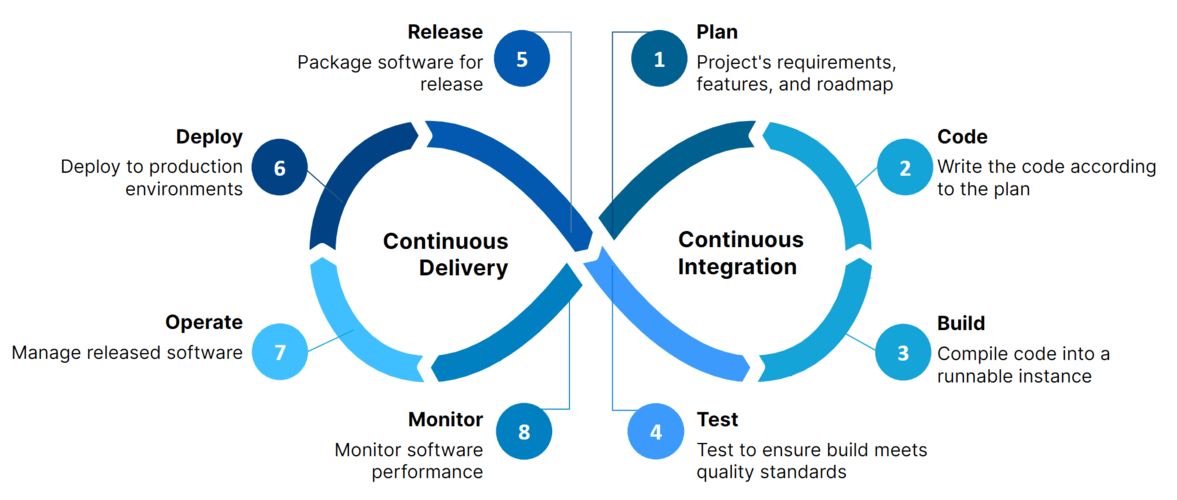
\includegraphics[keepaspectratio,alt={Vòng đời tổng quát của Continuous Integration và Continuous Delivery}]{images/cicdpipeline.png}}
\caption{Vòng đời tổng quát của Continuous Integration và Continuous
Delivery}
\end{figure}

Do đó, một pipeline tạo Docker image và cung cấp image đã kiểm chứng là
nền tảng cho Continuous Delivery; nó chưa đương nhiên là Continuous
Deployment. Hệ thống seminar dừng ở mức tích hợp liên tục, đóng gói và
kiểm chứng artifact. Không có bước tự động phát hành ứng dụng lên môi
trường production.

\section{2.4. Pipeline và quality
gate}\label{24-pipeline-vuxe0-quality-gate}

Pipeline là mô hình hóa một quy trình phân phối phần mềm thành các bước
có thứ tự hoặc quan hệ phụ thuộc. Trong Jenkins, Pipeline được mô tả như
code trong \texttt{Jenkinsfile}; GitHub Actions mô tả workflow, job và
step trong tệp YAML {[}4{]}, {[}5{]}.

Một \textbf{quality gate} là điều kiện phải đạt trước khi artifact được
chuyển sang giai đoạn sau. Ví dụ, nếu unit test trả exit code khác 0 thì
job thất bại và Docker image không được build. Các bước không làm thay
đổi quyết định pass/fail, chẳng hạn chỉ thu thập dữ liệu chẩn đoán,
không nên được gọi là quality gate.

Nguyên tắc \emph{fail-fast} cho phép dừng sớm các nhánh phụ thuộc khi
một điều kiện bắt buộc thất bại. Tuy nhiên, bước công bố report và log
vẫn nên chạy ở phần hậu xử lý, vì bằng chứng lỗi cần thiết chính trong
trường hợp pipeline thất bại.

\section{2.5. Test harness}\label{25-test-harness}

ISO/IEC/IEEE 24765 mô tả test harness như một hệ thống gồm test driver
và các công cụ hỗ trợ việc thực thi kiểm thử {[}6{]}. Trong thực tế, một
harness thường đảm nhiệm bốn nhóm trách nhiệm:

\begin{enumerate}
\def\labelenumi{\arabic{enumi}.}
\tightlist
\item
  \textbf{Thiết lập:} chuẩn bị runtime, dependency, database, dữ liệu và
  cấu hình.
\item
  \textbf{Điều khiển:} khởi động SUT, test runner, driver, stub hoặc
  probe theo đúng trình tự.
\item
  \textbf{Quan sát:} thu nhận response, assertion, exit code, log, ảnh
  chụp hoặc video.
\item
  \textbf{Kết thúc:} xuất report và khôi phục môi trường, kể cả khi kiểm
  thử thất bại.
\end{enumerate}

\begin{figure}
\centering
\pandocbounded{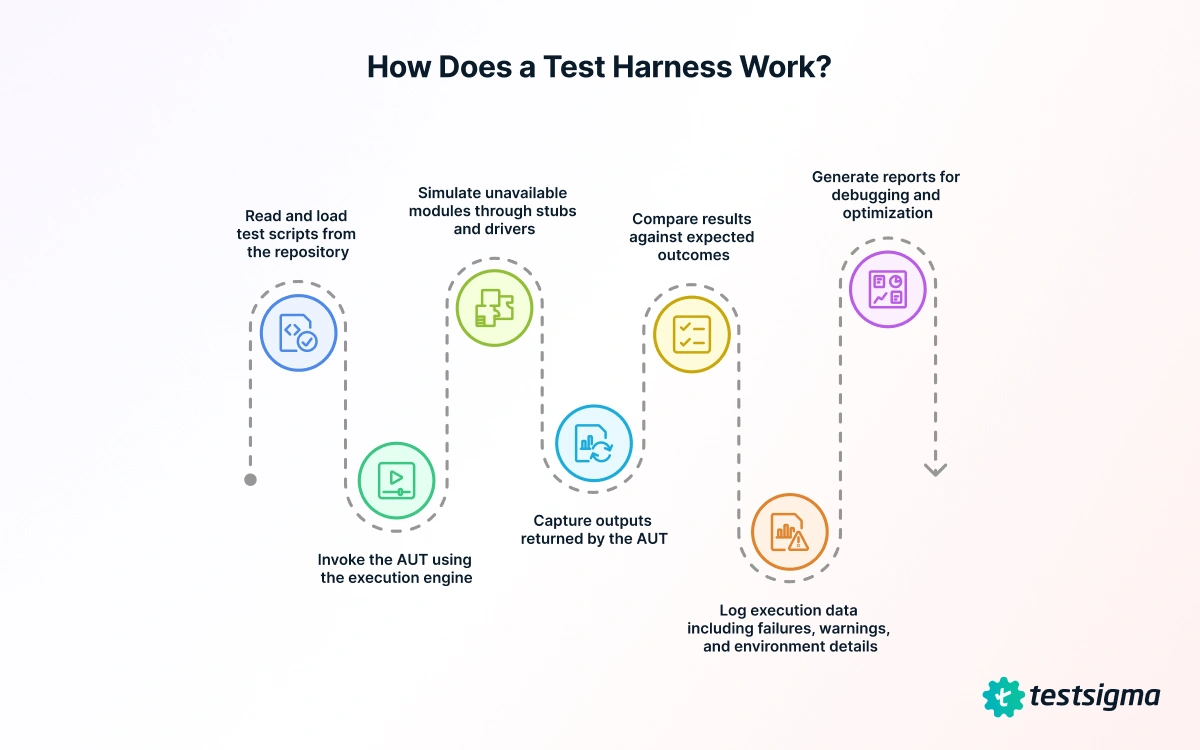
\includegraphics[keepaspectratio,alt={Các hoạt động chính của một test harness}]{images/How-Does-a-Test-Harness-Work.png}}
\caption{Các hoạt động chính của một test harness}
\end{figure}

Test harness không đồng nhất với test suite và cũng không đồng nhất với
CI pipeline. Test suite là tập hợp các ca kiểm thử. Test framework cung
cấp API và quy ước để viết test. Test runner khám phá và thực thi test.
Pipeline điều phối toàn bộ các hoạt động build, test và đóng gói.
Harness là phần môi trường và cơ chế giúp các test được chạy, quan sát
và lặp lại một cách kiểm soát.

\begin{longtable}[]{@{}
  >{\raggedright\arraybackslash}p{(\linewidth - 4\tabcolsep) * \real{0.2400}}
  >{\raggedright\arraybackslash}p{(\linewidth - 4\tabcolsep) * \real{0.3200}}
  >{\raggedright\arraybackslash}p{(\linewidth - 4\tabcolsep) * \real{0.4400}}@{}}
\toprule\noalign{}
\begin{minipage}[b]{\linewidth}\raggedright
Khái niệm
\end{minipage} & \begin{minipage}[b]{\linewidth}\raggedright
Chức năng
\end{minipage} & \begin{minipage}[b]{\linewidth}\raggedright
Ví dụ trong đề tài
\end{minipage} \\
\midrule\noalign{}
\endhead
\bottomrule\noalign{}
\endlastfoot
Test case & Một tập điều kiện, hành động và kết quả mong đợi & API không
có token phải trả \texttt{401} \\
Test suite & Nhóm các test case liên quan &
\texttt{tests/api/api.test.js} \\
Test framework/runner & API viết assertion và cơ chế thực thi test &
Jest, Mocha, Cypress \\
Test harness & Chuẩn bị SUT, điều khiển runner, thu kết quả và cleanup &
Script Jenkins, \texttt{image\_smoke.py}, cấu hình report \\
CI/CD pipeline & Điều phối build, test, artifact và luồng bàn giao &
GitHub Actions và Jenkinsfile \\
\end{longtable}

\section{2.6. Các mức kiểm
thử}\label{26-cuxe1c-mux1ee9c-kiux1ec3m-thux1eed}

Mức kiểm thử được xác định bởi phạm vi đối tượng và mục tiêu của phép
kiểm tra, không chỉ bởi tên công cụ.

\begin{itemize}
\tightlist
\item
  \textbf{Component/unit testing} kiểm tra một đơn vị nhỏ trong sự cô
  lập tương đối. Đề tài dùng Jest cho helper, middleware và hành vi của
  model.
\item
  \textbf{Integration testing} kiểm tra sự tương tác giữa các thành
  phần. SuperTest gửi HTTP request đến ứng dụng và kiểm tra sự phối hợp
  giữa route, middleware, model và database.
\item
  \textbf{System testing} đánh giá hệ thống đã tích hợp theo hành vi
  quan sát từ bên ngoài. Cypress điều khiển giao diện web thật và đồng
  thời quan sát request/response của API.
\end{itemize}

Mô hình \emph{test automation pyramid} khuyến nghị có nhiều kiểm tra
nhỏ, nhanh ở tầng thấp và ít kiểm tra xuyên hệ thống hơn ở tầng cao
{[}7{]}. Đây là một heuristic về chi phí và tốc độ phản hồi, không phải
một tỷ lệ bắt buộc. Cấu trúc 31 unit, 15 API và 5 UI tests của seminar
đi theo định hướng này.

\textbf{Smoke test} là một tập kiểm tra hẹp nhằm xác nhận các chức năng
quan trọng nhất đủ hoạt động để tiếp tục đánh giá sâu hơn. Trong đề tài,
\texttt{GET\ /api/tags} được dùng để xác nhận container có thể nhận
request và trả JSON đúng cấu trúc trước khi Cypress chạy.

\section{2.7. Báo cáo, sản phẩm đầu ra và khả năng truy
vết}\label{27-buxe1o-cuxe1o-sux1ea3n-phux1ea9m-ux111ux1ea7u-ra-vuxe0-khux1ea3-nux103ng-truy-vux1ebft}

\textbf{Báo cáo kiểm thử (test report)} biểu diễn kết quả thực thi: test
nào pass/fail, thời lượng và thông tin lỗi. \textbf{Sản phẩm đầu ra
(artifact)} là dữ liệu được lưu sau một lần chạy, có thể gồm báo cáo,
image, log, video và dữ liệu chẩn đoán. \textbf{Khả năng truy vết
(traceability)} là khả năng nối kết kết quả với đầu vào đã tạo ra nó.

Đề tài dùng JUnit XML làm định dạng trao đổi kết quả giữa test runner và
hệ thống CI; Allure chuyển raw results thành báo cáo HTML có khả năng
duyệt theo suite và test case. Docker image được gắn tag bằng full
40-character Git SHA. Nhờ đó, nhóm có thể đối chiếu source revision,
image, Jenkins build và report thay vì phụ thuộc vào tag biến đổi như
\texttt{latest}.

\chapter{3. ĐỐI TƯỢNG VÀ CÔNG NGHỆ NGHIÊN
CỨU}\label{3-ux111ux1ed1i-tux1b0ux1ee3ng-vuxe0-cuxf4ng-nghux1ec7-nghiuxean-cux1ee9u}

\section{3.1. System Under Test: RealWorld
Conduit}\label{31-system-under-test-realworld-conduit}

RealWorld là một ứng dụng mạng xã hội dạng blog, còn được gọi là
Conduit. Phiên bản được nhóm sử dụng là một ứng dụng monolithic gồm giao
diện Next.js/React, REST API Express, ORM Sequelize và SQLite ở cấu hình
phát triển. Các chức năng chính gồm đăng ký, đăng nhập, bài viết, bình
luận, hồ sơ và tag.

Ứng dụng khai báo Node.js \texttt{14.21.3} và npm \texttt{6.14.18}. Việc
dùng đúng runtime này là yêu cầu quan trọng vì source và một số
dependency đã cũ. Repository không có lockfile được commit, vì vậy
pipeline dùng \texttt{npm\ install} thay cho \texttt{npm\ ci}.

\section{3.2. GitHub Actions}\label{32-github-actions}

GitHub Actions là nền tảng tự động hóa gắn với repository GitHub.
Workflow được định nghĩa bằng YAML trong \texttt{.github/workflows/};
mỗi workflow gồm trigger, job và step {[}5{]}. Nhóm chọn công cụ này cho
tầng CI vì nó nhận trực tiếp sự kiện từ repository, hiển thị check trên
commit/pull request, cung cấp runner tạm thời và hỗ trợ artifact cũng
như GHCR.

\section{3.3. Jenkins}\label{33-jenkins}

Jenkins là máy chủ tự động hóa có hệ sinh thái plugin và mô hình
Pipeline as Code {[}4{]}. Trong seminar, Jenkins được đóng gói thành
custom Docker image để cố định plugin, Node.js, Docker CLI, Cypress và
các thư viện headless. Jenkins đảm nhiệm phần kiểm chứng có trạng thái
hơn: nhận tham số bàn giao, kéo image, quản lý vòng đời container, chạy
UI tests và công bố Allure Report.

Việc sử dụng cả GitHub Actions và Jenkins không nhằm chạy trùng cùng một
tác vụ. GitHub Actions tạo và kiểm tra artifact ở phía repository;
Jenkins kiểm chứng artifact đó trong một môi trường riêng và quản lý báo
cáo UI.

\section{3.4. Công cụ kiểm
thử}\label{34-cuxf4ng-cux1ee5-kiux1ec3m-thux1eed}

\begin{longtable}[]{@{}
  >{\raggedright\arraybackslash}p{(\linewidth - 2\tabcolsep) * \real{0.3200}}
  >{\raggedright\arraybackslash}p{(\linewidth - 2\tabcolsep) * \real{0.6800}}@{}}
\toprule\noalign{}
\begin{minipage}[b]{\linewidth}\raggedright
Công cụ
\end{minipage} & \begin{minipage}[b]{\linewidth}\raggedright
Vai trò trong đề tài
\end{minipage} \\
\midrule\noalign{}
\endhead
\bottomrule\noalign{}
\endlastfoot
Mocha & Chạy 4 regression tests có sẵn của ứng dụng \\
Jest & Chạy unit tests, mock dependency và đo coverage \\
SuperTest & Gửi request trực tiếp đến REST API trong bộ Jest API
tests \\
Newman & Chạy Postman collection của dự án RealWorld \\
Cypress & Điều khiển trình duyệt headless và kiểm tra luồng UI/API \\
npm audit & Phát hiện lỗ hổng đã biết trong cây dependency và chặn mức
High/Critical \\
CodeQL & Phân tích tĩnh mã nguồn JavaScript/TypeScript theo các mẫu truy
vấn bảo mật \\
JUnit XML & Định dạng kết quả để CI đọc và vẽ test trend \\
Allure & Tổng hợp raw result thành báo cáo HTML \\
\end{longtable}

\section{3.5. Công nghệ đóng gói và lưu
trữ}\label{35-cuxf4ng-nghux1ec7-ux111uxf3ng-guxf3i-vuxe0-lux1b0u-trux1eef}

Docker tạo một image ứng dụng độc lập từ source đã qua kiểm tra. GitHub
Container Registry lưu image theo tên
\texttt{ghcr.io/thu2005/realworld:\textless{}commit-sha\textgreater{}}.
Docker Compose khởi tạo Jenkins và volume \texttt{jenkins\_home}, nhờ đó
tài khoản, job và lịch sử build được giữ lại khi container Jenkins được
tạo lại.

\chapter{4. KIẾN TRÚC GIẢI
PHÁP}\label{4-kiux1ebfn-truxfac-giux1ea3i-phuxe1p}

\section{4.1. Yêu cầu thiết
kế}\label{41-yuxeau-cux1ea7u-thiux1ebft-kux1ebf}

Hệ thống được thiết kế theo các yêu cầu sau:

\begin{itemize}
\tightlist
\item
  Mỗi lần chạy phải xác định được revision của source và image.
\item
  Pipeline phải dùng đúng Node.js và npm mà ứng dụng khai báo.
\item
  Các bước lint, test và build bắt buộc phải làm pipeline thất bại khi
  không đạt.
\item
  Report và log phải được thu thập ngay cả khi kiểm thử thất bại.
\item
  Secret không xuất hiện trong source, log hoặc ảnh chụp.
\item
  Container và network tạm phải được dọn sau build.
\item
  Các thành viên có thể phát triển phân hệ độc lập nhưng phải tuân theo
  cùng tham số và đường dẫn đầu ra.
\end{itemize}

\section{4.2. Kiến trúc tổng
thể}\label{42-kiux1ebfn-truxfac-tux1ed5ng-thux1ec3}

\begin{figure}
\centering
\pandocbounded{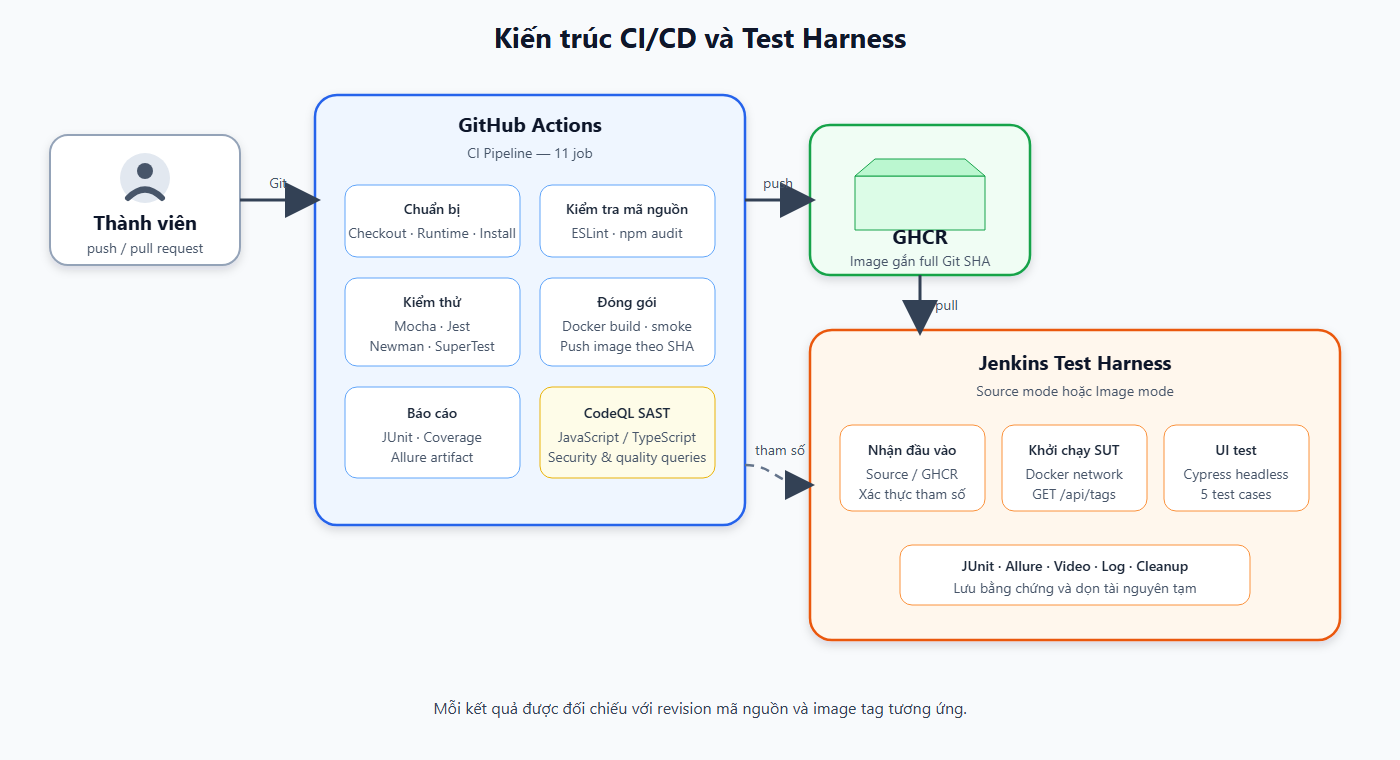
\includegraphics[keepaspectratio,alt={Kiến trúc CI/CD và Test Harness của đề tài}]{images/system-architecture.png}}
\caption{Kiến trúc CI/CD và Test Harness của đề tài}
\end{figure}

Kiến trúc có hai điểm kiểm soát. Điểm thứ nhất xác nhận source có thể
lint, test, build và đóng gói. Điểm thứ hai xác nhận chính image đã đóng
gói có thể chạy và phục vụ hành vi bên ngoài. Sự tách này giúp phát hiện
cả lỗi source lẫn lỗi chỉ xuất hiện sau containerization.

\section{4.3. Thiết kế workflow GitHub
Actions}\label{43-thiux1ebft-kux1ebf-workflow-github-actions}

Workflow \texttt{CI\ Pipeline} có 11 job. CodeQL được tách thành một
workflow riêng để có thể chạy theo sự kiện push, pull request, lịch hằng
tuần hoặc yêu cầu thủ công.

\begin{figure}
\centering
\pandocbounded{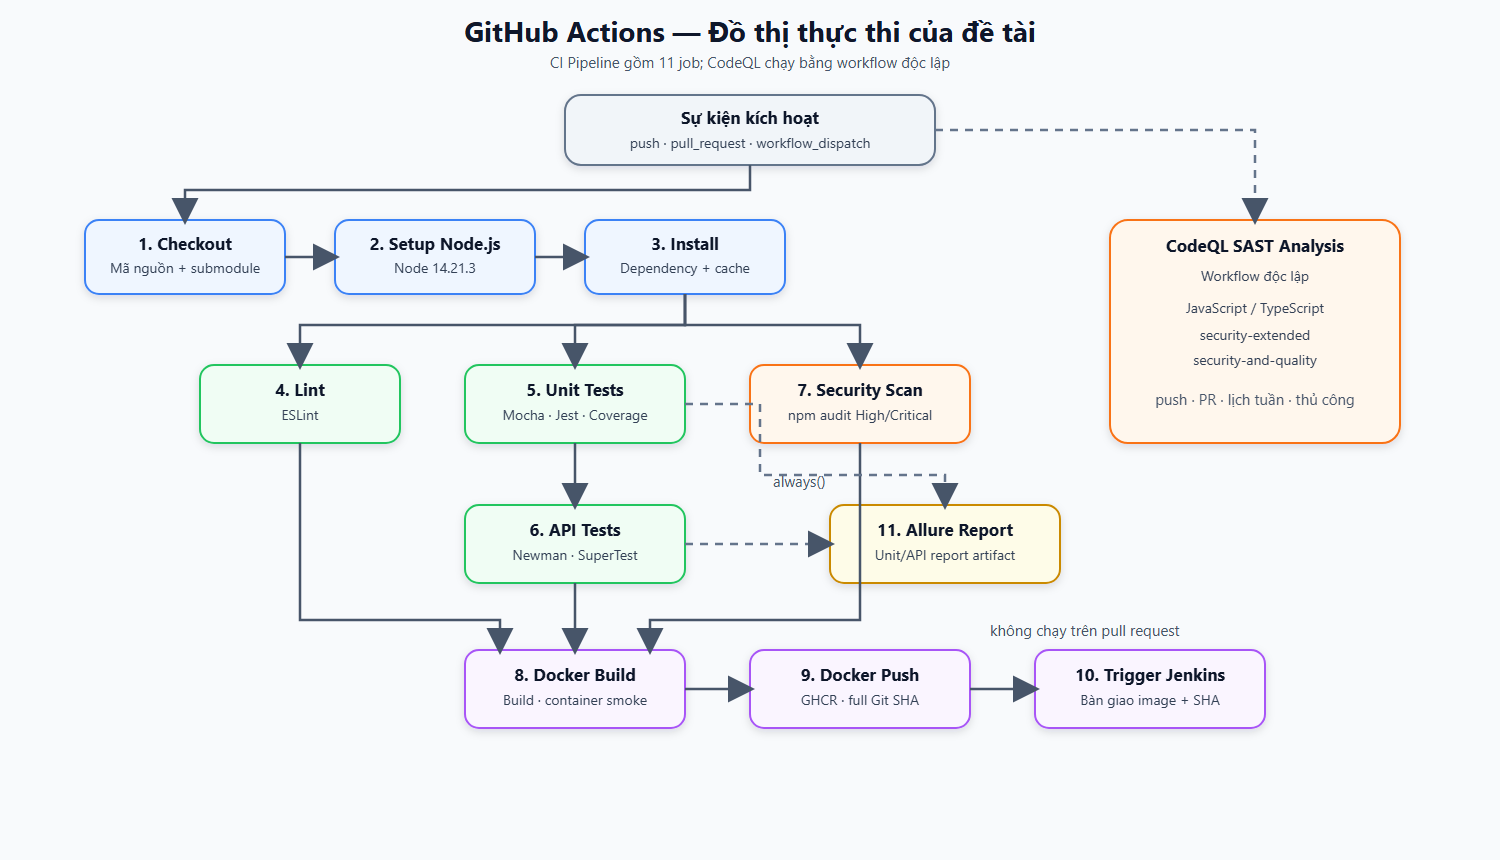
\includegraphics[keepaspectratio,alt={Đồ thị thực thi GitHub Actions của đề tài}]{images/github-actions-workflow.png}}
\caption{Đồ thị thực thi GitHub Actions của đề tài}
\end{figure}

\begin{longtable}[]{@{}
  >{\raggedleft\arraybackslash}p{(\linewidth - 4\tabcolsep) * \real{0.2400}}
  >{\raggedright\arraybackslash}p{(\linewidth - 4\tabcolsep) * \real{0.3200}}
  >{\raggedright\arraybackslash}p{(\linewidth - 4\tabcolsep) * \real{0.4400}}@{}}
\toprule\noalign{}
\begin{minipage}[b]{\linewidth}\raggedleft
Thứ tự logic
\end{minipage} & \begin{minipage}[b]{\linewidth}\raggedright
Job
\end{minipage} & \begin{minipage}[b]{\linewidth}\raggedright
Đầu ra/điều kiện chính
\end{minipage} \\
\midrule\noalign{}
\endhead
\bottomrule\noalign{}
\endlastfoot
1 & Checkout Repository & Source và submodule đúng revision \\
2 & Setup Node.js Runtime & Node \texttt{14.21.3} \\
3 & Install Dependencies & \texttt{node\_modules} được cache theo
\texttt{package.json} \\
4 & Lint Code & ESLint pass \\
5 & Unit Tests & Mocha XML và Jest coverage \\
6 & API Tests & Newman XML, server log và SuperTest result \\
7 & Security Vulnerability Scan & Lưu \texttt{security-audit.json}; dừng
pipeline nếu có mức High/Critical \\
8 & Docker Image Build & Image theo SHA và smoke test container pass \\
9 & Docker Image Push & Image được đẩy lên GHCR đối với sự kiện tin
cậy \\
10 & Trigger Jenkins Pipeline & Bàn giao thông tin image cho Jenkins \\
11 & Allure Report Dashboard & Tổng hợp report unit/API và lưu báo cáo
HTML dưới dạng artifact \\
\end{longtable}

Các job test và scan có thể chạy sau \texttt{install};
\texttt{docker-build} chỉ chạy sau lint, unit, API và security scan.
\texttt{docker-push} không chạy trên pull request vì pull request không
được phép phát hành package. Job Allure dùng
\texttt{always()\ \&\&\ !cancelled()} để vẫn thu báo cáo khi unit hoặc
API test thất bại. Workflow ghim các action bên thứ ba bằng commit SHA
và cấp \texttt{packages:\ write} riêng cho job cần đẩy image.

Workflow \texttt{CodeQL\ SAST\ Analysis} phân tích ngôn ngữ
\texttt{javascript-typescript} với hai bộ truy vấn
\texttt{security-extended} và \texttt{security-and-quality}. Job chỉ cấp
quyền \texttt{security-events:\ write} tại phạm vi cần thiết để gửi kết
quả phân tích lên GitHub Code Scanning.

\section{4.4. Thiết kế Jenkins
Pipeline}\label{44-thiux1ebft-kux1ebf-jenkins-pipeline}

Jenkinsfile hỗ trợ hai chế độ.

\begin{figure}
\centering
\pandocbounded{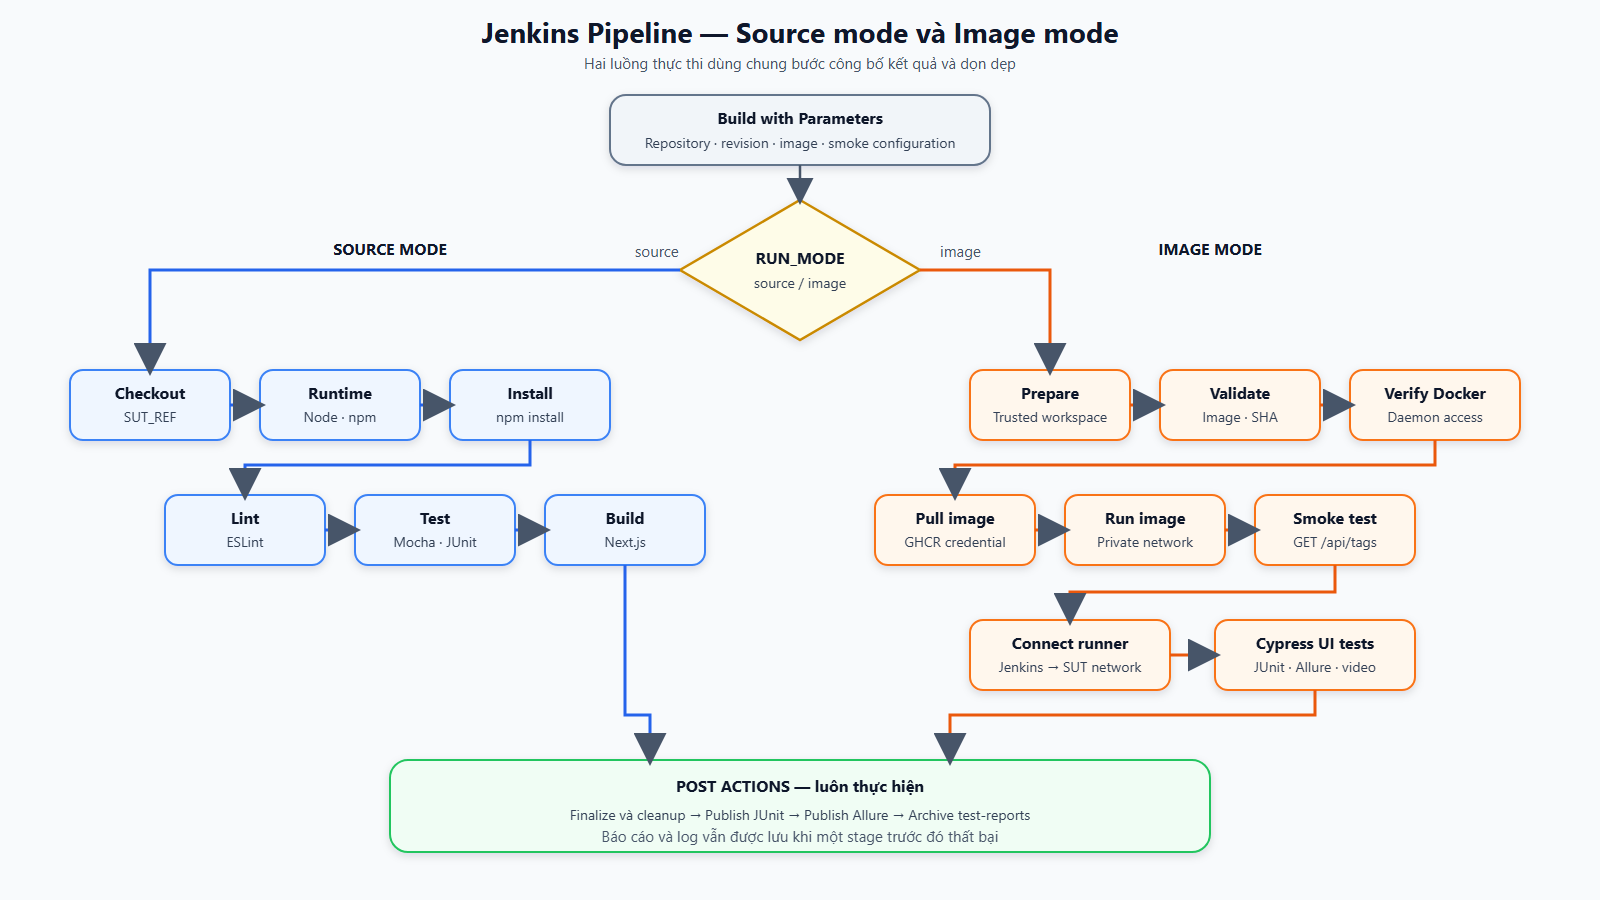
\includegraphics[keepaspectratio,alt={Hai chế độ thực thi của Jenkins Pipeline}]{images/jenkins-pipeline-workflow.png}}
\caption{Hai chế độ thực thi của Jenkins Pipeline}
\end{figure}

\subsection{4.4.1. Source mode}\label{441-source-mode}

\texttt{RUN\_MODE=source} thực hiện chuỗi:

\begin{Shaded}
\begin{Highlighting}[]
\NormalTok{Checkout {-}\textgreater{} Verify runtime {-}\textgreater{} Install {-}\textgreater{} Lint {-}\textgreater{} Mocha Test {-}\textgreater{} Build}
\end{Highlighting}
\end{Shaded}

Chế độ này là baseline độc lập. Jenkins có thể xác minh repository chỉ
với \texttt{SUT\_REPO\_URL} và \texttt{SUT\_REF}, hữu ích khi chưa có
Docker image hoặc cần kiểm tra trực tiếp source.

\subsection{4.4.2. Image mode}\label{442-image-mode}

\texttt{RUN\_MODE=image} thực hiện chuỗi:

\begin{Shaded}
\begin{Highlighting}[]
\NormalTok{Prepare {-}\textgreater{} Validate {-}\textgreater{} Verify Docker {-}\textgreater{} Pull image {-}\textgreater{} Run image}
\NormalTok{        {-}\textgreater{} Smoke test {-}\textgreater{} Connect UI runner {-}\textgreater{} Cypress UI tests}
\NormalTok{        {-}\textgreater{} Publish reports and cleanup}
\end{Highlighting}
\end{Shaded}

Image mode từ chối tag rỗng, tag \texttt{latest}, SHA sai định dạng hoặc
repository khác \texttt{ALLOWED\_IMAGE\_REPO}. Script
\texttt{jenkins/image\_smoke.py} tạo tên container và network theo
build, ghi label sở hữu, kiểm tra readiness có timeout và chỉ xóa tài
nguyên thuộc lần chạy hiện tại.

SUT không cần publish port ra host. Jenkins container được nối tạm vào
mạng riêng chứa SUT và truy cập bằng container name. Cách này tránh xung
đột host port và giảm bề mặt truy cập của ứng dụng trong lúc test.

\section{4.5. Quy ước tích hợp giữa các thành
phần}\label{45-quy-ux1b0ux1edbc-tuxedch-hux1ee3p-giux1eefa-cuxe1c-thuxe0nh-phux1ea7n}

Bốn tham số tạo thành giao diện bàn giao giữa hai hệ thống:

\begin{longtable}[]{@{}
  >{\raggedright\arraybackslash}p{(\linewidth - 2\tabcolsep) * \real{0.3200}}
  >{\raggedright\arraybackslash}p{(\linewidth - 2\tabcolsep) * \real{0.6800}}@{}}
\toprule\noalign{}
\begin{minipage}[b]{\linewidth}\raggedright
Tham số
\end{minipage} & \begin{minipage}[b]{\linewidth}\raggedright
Ý nghĩa
\end{minipage} \\
\midrule\noalign{}
\endhead
\bottomrule\noalign{}
\endlastfoot
\texttt{SUT\_REPO\_URL} & Repository chứa SUT \\
\texttt{SUT\_REF} & Branch, tag hoặc commit được kiểm tra ở source
mode \\
\texttt{IMAGE\_REPO} & Repository image, không gồm tag \\
\texttt{IMAGE\_TAG} & Full 40-character Git commit SHA \\
\end{longtable}

Các đầu ra được chuẩn hóa dưới \texttt{test-reports/}:

\begin{longtable}[]{@{}
  >{\raggedright\arraybackslash}p{(\linewidth - 2\tabcolsep) * \real{0.3200}}
  >{\raggedright\arraybackslash}p{(\linewidth - 2\tabcolsep) * \real{0.6800}}@{}}
\toprule\noalign{}
\begin{minipage}[b]{\linewidth}\raggedright
Loại đầu ra
\end{minipage} & \begin{minipage}[b]{\linewidth}\raggedright
Đường dẫn
\end{minipage} \\
\midrule\noalign{}
\endhead
\bottomrule\noalign{}
\endlastfoot
JUnit XML & \texttt{test-reports/junit/*.xml} \\
Allure raw results & \texttt{test-reports/allure-results/} \\
Cypress screenshots & \texttt{test-reports/cypress/screenshots/} \\
Cypress videos & \texttt{test-reports/cypress/videos/} \\
Runtime logs & \texttt{test-reports/logs/} \\
\end{longtable}

Các quy ước này giảm phụ thuộc giữa người viết test và người viết
pipeline: test runner có thể thay đổi nội bộ miễn là giữ command, điều
kiện pass/fail và output path đã thống nhất.

\section{4.6. Bảo vệ thông tin xác
thực}\label{46-bux1ea3o-vux1ec7-thuxf4ng-tin-xuxe1c-thux1ef1c}

GitHub Actions sử dụng \texttt{GITHUB\_TOKEN} theo phạm vi job để ghi
package. Các giá trị \texttt{JENKINS\_URL}, \texttt{JENKINS\_USER} và
\texttt{JENKINS\_TOKEN} được thiết kế để lấy từ GitHub Secrets. Jenkins
lưu thông tin GHCR private package bằng credential ID
\texttt{ghcr-credentials}; token được truyền cho \texttt{docker\ login}
qua standard input trong một \texttt{DOCKER\_CONFIG} tạm.

Mã nguồn chỉ chứa tên credential, không chứa giá trị bí mật. Thư mục cấu
hình Docker tạm được xóa sau khi pull, không nằm trong artifact. Đây là
ứng dụng của nguyên tắc phân tách cấu hình bí mật khỏi source và cấp
quyền tối thiểu theo nhu cầu.

\chapter{5. HIỆN THỰC TEST
HARNESS}\label{5-hiux1ec7n-thux1ef1c-test-harness}

\section{5.1. Cấu trúc hiện thực
chính}\label{51-cux1ea5u-truxfac-hiux1ec7n-thux1ef1c-chuxednh}

\begin{longtable}[]{@{}
  >{\raggedright\arraybackslash}p{(\linewidth - 2\tabcolsep) * \real{0.3200}}
  >{\raggedright\arraybackslash}p{(\linewidth - 2\tabcolsep) * \real{0.6800}}@{}}
\toprule\noalign{}
\begin{minipage}[b]{\linewidth}\raggedright
Tệp/thư mục
\end{minipage} & \begin{minipage}[b]{\linewidth}\raggedright
Trách nhiệm
\end{minipage} \\
\midrule\noalign{}
\endhead
\bottomrule\noalign{}
\endlastfoot
\texttt{.github/workflows/ci.yml} & Định nghĩa workflow GitHub
Actions \\
\texttt{.github/workflows/codeql.yml} & Định nghĩa workflow phân tích
tĩnh CodeQL \\
\texttt{Jenkinsfile} & Định nghĩa source mode, image mode và post
actions \\
\texttt{Dockerfile} & Đóng gói ứng dụng RealWorld \\
\texttt{docker-compose.jenkins.yml} & Khởi tạo Jenkins và volume dữ
liệu \\
\texttt{jenkins/Dockerfile} & Tạo Jenkins image có Node, Docker CLI và
Cypress \\
\texttt{jenkins/plugins.txt} & Danh sách plugin Jenkins tối thiểu \\
\texttt{jenkins/image\_smoke.py} & Quản lý vòng đời SUT container và
smoke test \\
\texttt{jenkins/trigger\_jenkins.py} & Client gọi Jenkins API và theo
dõi kết quả \\
\texttt{tests/unit/} & Jest unit test suites \\
\texttt{tests/api/} & SuperTest API integration suite \\
\texttt{cypress/e2e/} & Cypress UI/system tests \\
\texttt{CI\_INTEGRATION\_CONTRACT.md} & Quy ước tích hợp giữa các phân
hệ \\
\end{longtable}

\section{5.2. Môi trường Jenkins tái lập bằng
Docker}\label{52-muxf4i-trux1b0ux1eddng-jenkins-tuxe1i-lux1eadp-bux1eb1ng-docker}

Custom Jenkins image kế thừa \texttt{jenkins/jenkins:lts-jdk21}. Image
bổ sung:

\begin{itemize}
\tightlist
\item
  Node.js \texttt{14.21.3} và npm \texttt{6.14.18} cho source pipeline;
\item
  Docker CLI để Jenkins điều khiển container trên Docker daemon của
  host;
\item
  Python 3 cho các script tích hợp;
\item
  Cypress \texttt{9.7.0}, Allure adapter và thư viện Linux cho trình
  duyệt headless;
\item
  các plugin Pipeline, Git, credentials-binding, JUnit và Allure.
\end{itemize}

Danh sách plugin được cài trong quá trình build image, không phụ thuộc
vào thao tác ``Install suggested plugins'' trên giao diện. Groovy init
script tạo Allure command-line tool tên \texttt{allure} nếu cấu hình này
chưa tồn tại.

Compose ánh xạ Jenkins tới \texttt{127.0.0.1:18080}, gắn named volume
vào \texttt{/var/jenkins\_home} và gắn Docker socket. Việc gắn socket
cho phép Jenkins quản lý container nhưng cũng trao quyền lớn đối với
Docker host; vì vậy cấu hình này chỉ phù hợp với job tin cậy trong môi
trường seminar.

\section{5.3. Unit test bằng Jest}\label{53-unit-test-bux1eb1ng-jest}

Bộ unit test gồm 31 ca:

\begin{longtable}[]{@{}
  >{\raggedright\arraybackslash}p{(\linewidth - 4\tabcolsep) * \real{0.2400}}
  >{\raggedleft\arraybackslash}p{(\linewidth - 4\tabcolsep) * \real{0.3200}}
  >{\raggedright\arraybackslash}p{(\linewidth - 4\tabcolsep) * \real{0.4400}}@{}}
\toprule\noalign{}
\begin{minipage}[b]{\linewidth}\raggedright
Suite
\end{minipage} & \begin{minipage}[b]{\linewidth}\raggedleft
Số ca
\end{minipage} & \begin{minipage}[b]{\linewidth}\raggedright
Nội dung chính
\end{minipage} \\
\midrule\noalign{}
\endhead
\bottomrule\noalign{}
\endlastfoot
\texttt{lib.test.js} & 16 & Validate số nguyên/tham số, lỗi validation,
client IP, tag và cleanup dữ liệu demo \\
\texttt{auth.test.js} & 6 & Middleware bắt buộc/tùy chọn, header
Token/Bearer và trường hợp thiếu token \\
\texttt{models.test.js} & 9 & Hash mật khẩu, JWT, chuẩn hóa user,
validation và slug bài viết \\
\end{longtable}

Jest chạy trong môi trường Node và đặt threshold toàn cục 80\% cho
statements, branches, functions và lines. Tuy nhiên, cấu hình
\texttt{collectCoverageFrom} chỉ đo \texttt{lib.js} và \texttt{auth.js};
vì vậy số coverage trong báo cáo phải được hiểu là coverage của hai
mô-đun mục tiêu, không phải toàn bộ codebase.

\section{5.4. API test bằng SuperTest và
Newman}\label{54-api-test-bux1eb1ng-supertest-vuxe0-newman}

SuperTest suite gồm 15 ca kiểm tra REST API ở mức tích hợp. Các nhóm
hành vi chính là:

\begin{itemize}
\tightlist
\item
  \texttt{GET\ /api/tags} và cấu trúc response;
\item
  đăng ký, đăng nhập, JWT và truy cập không xác thực;
\item
  tạo và truy vấn bài viết;
\item
  profile và comment;
\item
  các mã lỗi \texttt{401}, \texttt{404} và \texttt{422}.
\end{itemize}

API tests chạy tuần tự để tránh dữ liệu dùng chung gây xung đột. Trước
Newman, workflow đồng bộ database, khởi động server nền và chờ
\texttt{GET\ /api/tags} phản hồi. Newman sau đó chạy collection của
submodule \texttt{realworld}, xuất kết quả JUnit XML. Hai bộ test bổ
sung cho nhau: SuperTest thể hiện các case nhóm chủ động viết, còn
Newman tái sử dụng contract collection của dự án RealWorld.

\section{5.5. UI test bằng Cypress}\label{55-ui-test-bux1eb1ng-cypress}

Cypress suite hiện có 5 ca trong hai spec:

\begin{longtable}[]{@{}
  >{\raggedright\arraybackslash}p{(\linewidth - 4\tabcolsep) * \real{0.2400}}
  >{\raggedleft\arraybackslash}p{(\linewidth - 4\tabcolsep) * \real{0.3200}}
  >{\raggedright\arraybackslash}p{(\linewidth - 4\tabcolsep) * \real{0.4400}}@{}}
\toprule\noalign{}
\begin{minipage}[b]{\linewidth}\raggedright
Spec
\end{minipage} & \begin{minipage}[b]{\linewidth}\raggedleft
Số ca
\end{minipage} & \begin{minipage}[b]{\linewidth}\raggedright
Hành vi
\end{minipage} \\
\midrule\noalign{}
\endhead
\bottomrule\noalign{}
\endlastfoot
\texttt{public-ui.spec.js} & 2 & Trang chủ và điều hướng đến form đăng
nhập \\
\texttt{account-validation.spec.js} & 3 & Thiếu mật khẩu, sai thông tin
đăng nhập và đăng ký thiếu mật khẩu \\
\end{longtable}

Các case chạy trên trình duyệt headless với viewport \texttt{1280x720}.
Test dùng DOM assertion để kiểm tra nội dung và điều hướng; các case
validation dùng \texttt{cy.intercept}/\texttt{cy.wait} để xác nhận đồng
thời HTTP status \texttt{422} và thông báo lỗi trên UI. Video luôn được
ghi; screenshot được tạo khi test lỗi. Allure adapter ghi raw results để
Jenkins công bố báo cáo.

\section{5.6. Container smoke test và
cleanup}\label{56-container-smoke-test-vuxe0-cleanup}

Sau khi image được kéo về, harness lưu image ID/digest, tạo một network
riêng và chạy SUT bằng image ID đã xác định. Một probe container gọi
\texttt{GET\ /api/tags} với số lần thử và timeout hữu hạn. Phép kiểm tra
chỉ pass khi nhận HTTP \texttt{200} và body JSON có mảng \texttt{tags}.

Post action thu thập \texttt{container.log},
\texttt{container-inspect.json}, \texttt{smoke-response.json},
\texttt{integration-summary.json} và \texttt{smoke.xml}. Cuối cùng,
Jenkins ngắt kết nối khỏi network rồi xóa app container, probe container
và network mang label của build. Cleanup được đặt trong hậu xử lý để vẫn
chạy khi smoke test hoặc Cypress thất bại.

\section{5.7. Báo cáo kiểm thử và kiểm tra bảo mật trên GitHub
Actions}\label{57-buxe1o-cuxe1o-kiux1ec3m-thux1eed-vuxe0-kiux1ec3m-tra-bux1ea3o-mux1eadt-truxean-github-actions}

Phần hiện thực GitHub Actions tại revision \texttt{19c70a9} mở rộng
pipeline theo ba hướng.

Thứ nhất, \texttt{jest-junit} được cấu hình làm reporter của Jest. Unit
tests ghi \texttt{jest-unit.xml}, API tests ghi \texttt{jest-api.xml};
coverage được xuất ở ba dạng \texttt{text}, \texttt{lcov} và
\texttt{json-summary}. Workflow đọc \texttt{coverage-summary.json} để
tạo bảng statements, branches, functions và lines ngay trong GitHub
Actions Job Summary. Các tệp XML và thư mục coverage đồng thời được lưu
thành artifact.

Thứ hai, job \texttt{security-scan} tạo \texttt{security-audit.json},
trình bày số lỗ hổng theo năm mức độ và thực thi
\texttt{npm\ audit\ -\/-audit-level=high}. Lệnh này trả trạng thái thất
bại khi cây dependency còn lỗ hổng High hoặc Critical, vì vậy kết quả
kiểm tra bảo mật tham gia trực tiếp vào quyết định có cho phép
\texttt{docker-build} chạy hay không.

Thứ ba, workflow \texttt{CodeQL\ SAST\ Analysis} phân tích tĩnh mã
JavaScript/TypeScript bằng các bộ truy vấn mở rộng về bảo mật và chất
lượng. Workflow chạy khi có thay đổi mã nguồn, trên pull request, theo
lịch hằng tuần và khi được kích hoạt thủ công. Bên cạnh đó, job
\texttt{allure-report} tải artifact của unit/API tests, tổng hợp dữ liệu
đầu vào và tạo artifact HTML \texttt{allure-report-dashboard} với thời
gian lưu 7 ngày. README của nhánh cũng hiển thị trạng thái pipeline, số
unit/API tests và coverage để người xem nhận biết nhanh trạng thái kiểm
thử gần nhất.

\chapter{6. TRIỂN KHAI HẠ TẦNG VÀ TÁI HIỆN THỰC
NGHIỆM}\label{6-triux1ec3n-khai-hux1ea1-tux1ea7ng-vuxe0-tuxe1i-hiux1ec7n-thux1ef1c-nghiux1ec7m}

Chương này mô tả quy trình đã dùng để triển khai môi trường seminar. Các
lệnh được chạy trong Linux hoặc WSL2 có Docker Engine/Docker Desktop
integration.

\section{6.1. Điều kiện môi
trường}\label{61-ux111iux1ec1u-kiux1ec7n-muxf4i-trux1b0ux1eddng}

\begin{itemize}
\tightlist
\item
  Git hỗ trợ submodule;
\item
  Docker Engine và Docker Compose v2;
\item
  tối thiểu khoảng 8 GB RAM để build ứng dụng, Jenkins và Cypress;
\item
  quyền truy cập repository GitHub và GHCR tương ứng;
\item
  cổng host \texttt{18080} chưa được sử dụng.
\end{itemize}

\section{6.2. Lấy mã nguồn}\label{62-lux1ea5y-muxe3-nguux1ed3n}

\begin{Shaded}
\begin{Highlighting}[]
\FunctionTok{git}\NormalTok{ clone }\AttributeTok{{-}{-}recurse{-}submodules}\NormalTok{ https://github.com/thu2005/realworld.git}
\BuiltInTok{cd}\NormalTok{ realworld}
\FunctionTok{git}\NormalTok{ checkout next}
\FunctionTok{git}\NormalTok{ submodule update }\AttributeTok{{-}{-}init} \AttributeTok{{-}{-}recursive}
\FunctionTok{git}\NormalTok{ rev{-}parse HEAD}
\end{Highlighting}
\end{Shaded}

Lệnh cuối ghi nhận revision được dùng trong thực nghiệm. Khi tái hiện
một kết quả cũ, cần checkout đúng commit thay vì chỉ dựa vào tên branch
có thể thay đổi.

\section{6.3. Build và khởi động
Jenkins}\label{63-build-vuxe0-khux1edfi-ux111ux1ed9ng-jenkins}

\begin{Shaded}
\begin{Highlighting}[]
\ExtensionTok{docker}\NormalTok{ compose }\AttributeTok{{-}f}\NormalTok{ docker{-}compose.jenkins.yml config }\AttributeTok{{-}{-}quiet}
\ExtensionTok{docker}\NormalTok{ compose }\AttributeTok{{-}f}\NormalTok{ docker{-}compose.jenkins.yml build jenkins}
\ExtensionTok{docker}\NormalTok{ compose }\AttributeTok{{-}f}\NormalTok{ docker{-}compose.jenkins.yml up }\AttributeTok{{-}d} \AttributeTok{{-}{-}no{-}build}\NormalTok{ jenkins}
\ExtensionTok{docker}\NormalTok{ compose }\AttributeTok{{-}f}\NormalTok{ docker{-}compose.jenkins.yml ps}
\end{Highlighting}
\end{Shaded}

Giao diện Jenkins được mở tại \texttt{http://localhost:18080}. Named
volume \texttt{jenkins\_home} được giữ qua các lần recreate container.
Sau khi khởi động, khả năng truy cập Docker và Cypress được xác nhận
bằng:

\begin{Shaded}
\begin{Highlighting}[]
\ExtensionTok{docker}\NormalTok{ compose }\AttributeTok{{-}f}\NormalTok{ docker{-}compose.jenkins.yml exec jenkins docker version}
\ExtensionTok{docker}\NormalTok{ compose }\AttributeTok{{-}f}\NormalTok{ docker{-}compose.jenkins.yml exec jenkins cypress verify}
\end{Highlighting}
\end{Shaded}

\section{6.4. Tạo Pipeline job}\label{64-tux1ea1o-pipeline-job}

Trong Jenkins, nhóm tạo job loại \textbf{Pipeline} với tên
\texttt{ci-cd-demo}, chọn \textbf{Pipeline script from SCM}, sau đó cấu
hình:

\begin{longtable}[]{@{}
  >{\raggedright\arraybackslash}p{(\linewidth - 2\tabcolsep) * \real{0.3200}}
  >{\raggedright\arraybackslash}p{(\linewidth - 2\tabcolsep) * \real{0.6800}}@{}}
\toprule\noalign{}
\begin{minipage}[b]{\linewidth}\raggedright
Thuộc tính
\end{minipage} & \begin{minipage}[b]{\linewidth}\raggedright
Giá trị
\end{minipage} \\
\midrule\noalign{}
\endhead
\bottomrule\noalign{}
\endlastfoot
SCM & Git \\
Repository URL & \texttt{https://github.com/thu2005/realworld.git} \\
Branch Specifier & \texttt{*/next} \\
Script Path & \texttt{Jenkinsfile} \\
\end{longtable}

Lần chạy đầu tiên nạp Jenkinsfile và tạo danh sách tham số; các lần sau
giao diện hiển thị \textbf{Build with Parameters}.

\section{6.5. Cấu hình credential
GHCR}\label{65-cux1ea5u-huxecnh-credential-ghcr}

Đối với package private, một credential loại \textbf{Username with
password} được tạo trong Jenkins:

\begin{longtable}[]{@{}
  >{\raggedright\arraybackslash}p{(\linewidth - 2\tabcolsep) * \real{0.3200}}
  >{\raggedright\arraybackslash}p{(\linewidth - 2\tabcolsep) * \real{0.6800}}@{}}
\toprule\noalign{}
\begin{minipage}[b]{\linewidth}\raggedright
Trường
\end{minipage} & \begin{minipage}[b]{\linewidth}\raggedright
Giá trị
\end{minipage} \\
\midrule\noalign{}
\endhead
\bottomrule\noalign{}
\endlastfoot
ID & \texttt{ghcr-credentials} \\
Username & Tài khoản GitHub có quyền đọc package \\
Password & Personal access token có quyền đọc package \\
\end{longtable}

Token chỉ được nhập vào Jenkins Credentials. Pipeline tham chiếu
credential qua ID và không ghi token vào \texttt{Jenkinsfile}.

\section{6.6. Chạy source mode}\label{66-chux1ea1y-source-mode}

Các tham số chính:

\begin{longtable}[]{@{}
  >{\raggedright\arraybackslash}p{(\linewidth - 2\tabcolsep) * \real{0.3200}}
  >{\raggedright\arraybackslash}p{(\linewidth - 2\tabcolsep) * \real{0.6800}}@{}}
\toprule\noalign{}
\begin{minipage}[b]{\linewidth}\raggedright
Tham số
\end{minipage} & \begin{minipage}[b]{\linewidth}\raggedright
Giá trị mẫu
\end{minipage} \\
\midrule\noalign{}
\endhead
\bottomrule\noalign{}
\endlastfoot
\texttt{RUN\_MODE} & \texttt{source} \\
\texttt{SUT\_REPO\_URL} &
\texttt{https://github.com/thu2005/realworld.git} \\
\texttt{SUT\_REF} & \texttt{next} hoặc một full commit SHA \\
\end{longtable}

Sau khi build kết thúc, Stage View phải thể hiện các bước checkout,
runtime, install, lint, test và build. \texttt{SUT\_REF} nên là commit
SHA khi cần tái hiện chính xác một kết quả.

\section{6.7. Chạy image mode}\label{67-chux1ea1y-image-mode}

Các tham số dùng để kiểm chứng GHCR image:

\begin{longtable}[]{@{}
  >{\raggedright\arraybackslash}p{(\linewidth - 2\tabcolsep) * \real{0.3200}}
  >{\raggedright\arraybackslash}p{(\linewidth - 2\tabcolsep) * \real{0.6800}}@{}}
\toprule\noalign{}
\begin{minipage}[b]{\linewidth}\raggedright
Tham số
\end{minipage} & \begin{minipage}[b]{\linewidth}\raggedright
Giá trị
\end{minipage} \\
\midrule\noalign{}
\endhead
\bottomrule\noalign{}
\endlastfoot
\texttt{RUN\_MODE} & \texttt{image} \\
\texttt{IMAGE\_REPO} & \texttt{ghcr.io/thu2005/realworld} \\
\texttt{IMAGE\_TAG} & full 40-character commit SHA \\
\texttt{PULL\_IMAGE} & \texttt{true} \\
\texttt{GHCR\_PRIVATE} & \texttt{true} khi package private \\
\texttt{SMOKE\_TIMEOUT\_SECONDS} & \texttt{120} \\
\texttt{SMOKE\_PATH} & \texttt{/api/tags} \\
\end{longtable}

Tag image phải tương ứng với commit mà GitHub Actions đã dùng để build.
Khi pipeline hoàn tất, giao diện Jenkins cung cấp Test Result, Allure
Report và Build Artifacts. Không cần mở port của SUT ra host vì các phép
kiểm tra chạy trong mạng Docker nội bộ.

\section{6.8. Kiểm tra report và trạng thái
cleanup}\label{68-kiux1ec3m-tra-report-vuxe0-trux1ea1ng-thuxe1i-cleanup}

Các bằng chứng quan trọng sau một image-mode build gồm:

\begin{itemize}
\tightlist
\item
  JUnit result của smoke test và Cypress;
\item
  Allure Report;
\item
  Cypress video hoặc screenshot;
\item
  image reference, image ID/digest và source SHA trong integration
  summary;
\item
  log container;
\item
  kết quả cleanup.
\end{itemize}

Có thể kiểm tra không còn tài nguyên tạm bằng \texttt{docker\ ps\ -a} và
\texttt{docker\ network\ ls}. Harness không dùng lệnh prune toàn cục; nó
chỉ xóa tài nguyên có nhãn sở hữu của build.

\chapter{7. PHÂN TÍCH BỘ KIỂM
THỬ}\label{7-phuxe2n-tuxedch-bux1ed9-kiux1ec3m-thux1eed}

\section{7.1. Phân bố kiểm
thử}\label{71-phuxe2n-bux1ed1-kiux1ec3m-thux1eed}

\begin{longtable}[]{@{}
  >{\raggedright\arraybackslash}p{(\linewidth - 6\tabcolsep) * \real{0.2000}}
  >{\raggedright\arraybackslash}p{(\linewidth - 6\tabcolsep) * \real{0.2000}}
  >{\raggedleft\arraybackslash}p{(\linewidth - 6\tabcolsep) * \real{0.2000}}
  >{\raggedright\arraybackslash}p{(\linewidth - 6\tabcolsep) * \real{0.4000}}@{}}
\toprule\noalign{}
\begin{minipage}[b]{\linewidth}\raggedright
Mức/loại kiểm thử
\end{minipage} & \begin{minipage}[b]{\linewidth}\raggedright
Công cụ
\end{minipage} & \begin{minipage}[b]{\linewidth}\raggedleft
Số ca đếm trực tiếp
\end{minipage} & \begin{minipage}[b]{\linewidth}\raggedright
Mục tiêu
\end{minipage} \\
\midrule\noalign{}
\endhead
\bottomrule\noalign{}
\endlastfoot
Regression có sẵn & Mocha & 4 & Xác nhận hành vi nền của ứng dụng \\
Unit & Jest & 31 & Helper, auth middleware và model \\
API integration & SuperTest & 15 & Các API REST và luồng dữ liệu \\
API contract collection & Newman & Theo collection & Kiểm tra RealWorld
API contract \\
UI/system & Cypress & 5 & Điều hướng và validation qua giao diện \\
\end{longtable}

Nếu chỉ tính các case được khai báo trực tiếp trong source của
repository, hệ thống có 55 test cases. Newman được báo cáo riêng vì số
iteration/request do collection và script của submodule quyết định; cộng
nó vào một tổng tĩnh dễ tạo số liệu sai.

\section{7.2. Mức độ bao phủ hành
vi}\label{72-mux1ee9c-ux111ux1ed9-bao-phux1ee7-huxe0nh-vi}

Bộ unit test tập trung vào logic có thể cô lập và thực thi nhanh. API
suite mở rộng sang authentication, bài viết, profile và comment. UI
suite kiểm tra đường đi công khai và ba trường hợp validation tài khoản.
Cấu trúc này tạo ba lớp phản hồi: lỗi hàm/middleware được phát hiện
nhanh ở Jest; lỗi tích hợp route và database được phát hiện ở API; lỗi
nối kết giữa browser, UI và backend được phát hiện ở Cypress.

\section{7.3. Phân tích coverage}\label{73-phuxe2n-tuxedch-coverage}

Kết quả Jest trên hai tệp được cấu hình đo coverage:

\begin{longtable}[]{@{}
  >{\raggedright\arraybackslash}p{(\linewidth - 4\tabcolsep) * \real{0.2400}}
  >{\raggedleft\arraybackslash}p{(\linewidth - 4\tabcolsep) * \real{0.3200}}
  >{\raggedleft\arraybackslash}p{(\linewidth - 4\tabcolsep) * \real{0.4400}}@{}}
\toprule\noalign{}
\begin{minipage}[b]{\linewidth}\raggedright
Chỉ số
\end{minipage} & \begin{minipage}[b]{\linewidth}\raggedleft
Kết quả
\end{minipage} & \begin{minipage}[b]{\linewidth}\raggedleft
Threshold
\end{minipage} \\
\midrule\noalign{}
\endhead
\bottomrule\noalign{}
\endlastfoot
Statements & 100\% & 80\% \\
Branches & 94,73\% & 80\% \\
Functions & 100\% & 80\% \\
Lines & 100\% & 80\% \\
\end{longtable}

Coverage là chỉ báo về phần cấu trúc mã đã được thực thi, không tự chứng
minh rằng mọi yêu cầu hay mọi lỗi đều đã được kiểm tra. Giá trị của kết
quả trên nằm ở việc hai mô-đun mục tiêu vượt threshold và pipeline có
thể tự động phát hiện regression coverage. Nó không được dùng để kết
luận toàn bộ RealWorld đạt 100\% coverage.

\section{7.4. Oracle và khả năng chẩn
đoán}\label{74-oracle-vuxe0-khux1ea3-nux103ng-chux1ea9n-ux111ouxe1n}

Các suite dùng nhiều dạng oracle:

\begin{itemize}
\tightlist
\item
  giá trị trả về và exception đối với unit test;
\item
  HTTP status và JSON body đối với API/smoke test;
\item
  DOM state, URL, HTTP status và thông báo lỗi đối với Cypress;
\item
  exit code để truyền trạng thái pass/fail cho pipeline.
\end{itemize}

Khi thất bại, JUnit XML xác định test case và message; server/container
log cho biết lỗi runtime; Cypress video/screenshot giúp quan sát trạng
thái UI; Allure nhóm kết quả theo suite. Việc kết hợp oracle với
artifact chẩn đoán làm giảm thời gian xác định lỗi so với chỉ lưu
console output.

\chapter{8. THỰC NGHIỆM VÀ KẾT
QUẢ}\label{8-thux1ef1c-nghiux1ec7m-vuxe0-kux1ebft-quux1ea3}

\section{8.1. Thiết kế thực
nghiệm}\label{81-thiux1ebft-kux1ebf-thux1ef1c-nghiux1ec7m}

Nhóm kiểm chứng bốn câu hỏi:

\begin{enumerate}
\def\labelenumi{\arabic{enumi}.}
\tightlist
\item
  Source có vượt qua các kiểm tra lint, unit, API và build trên CI hay
  không?
\item
  Docker image có khởi động và phản hồi API kiểm tra tối thiểu hay
  không?
\item
  Jenkins có nhận đúng image theo commit SHA, chạy Cypress và xuất
  report hay không?
\item
  Sau build, artifact có được lưu và tài nguyên tạm có được dọn hay
  không?
\end{enumerate}

Đầu vào chính là nhánh \texttt{next}; runner GitHub Actions dùng Ubuntu;
Jenkins chạy trong Docker trên môi trường local/WSL2. Kết quả được đánh
giá từ trạng thái job, test report, Allure, artifact list và ảnh chụp
màn hình.

\section{8.2. Kết quả GitHub
Actions}\label{82-kux1ebft-quux1ea3-github-actions}

Tại merge commit \texttt{4f9a9405b2baebc42969d40f638501e8debfd20e},
GitHub hiển thị \textbf{10 successful checks}. Các job API Tests, Unit
Tests, Lint Code, Docker Image Build, Docker Image Push và Trigger
Jenkins Pipeline đều thành công. Kết quả này xác nhận chuỗi từ source
đến GHCR image đã chạy hoàn chỉnh trên sự kiện push vào \texttt{next}.

\begin{figure}
\centering
\pandocbounded{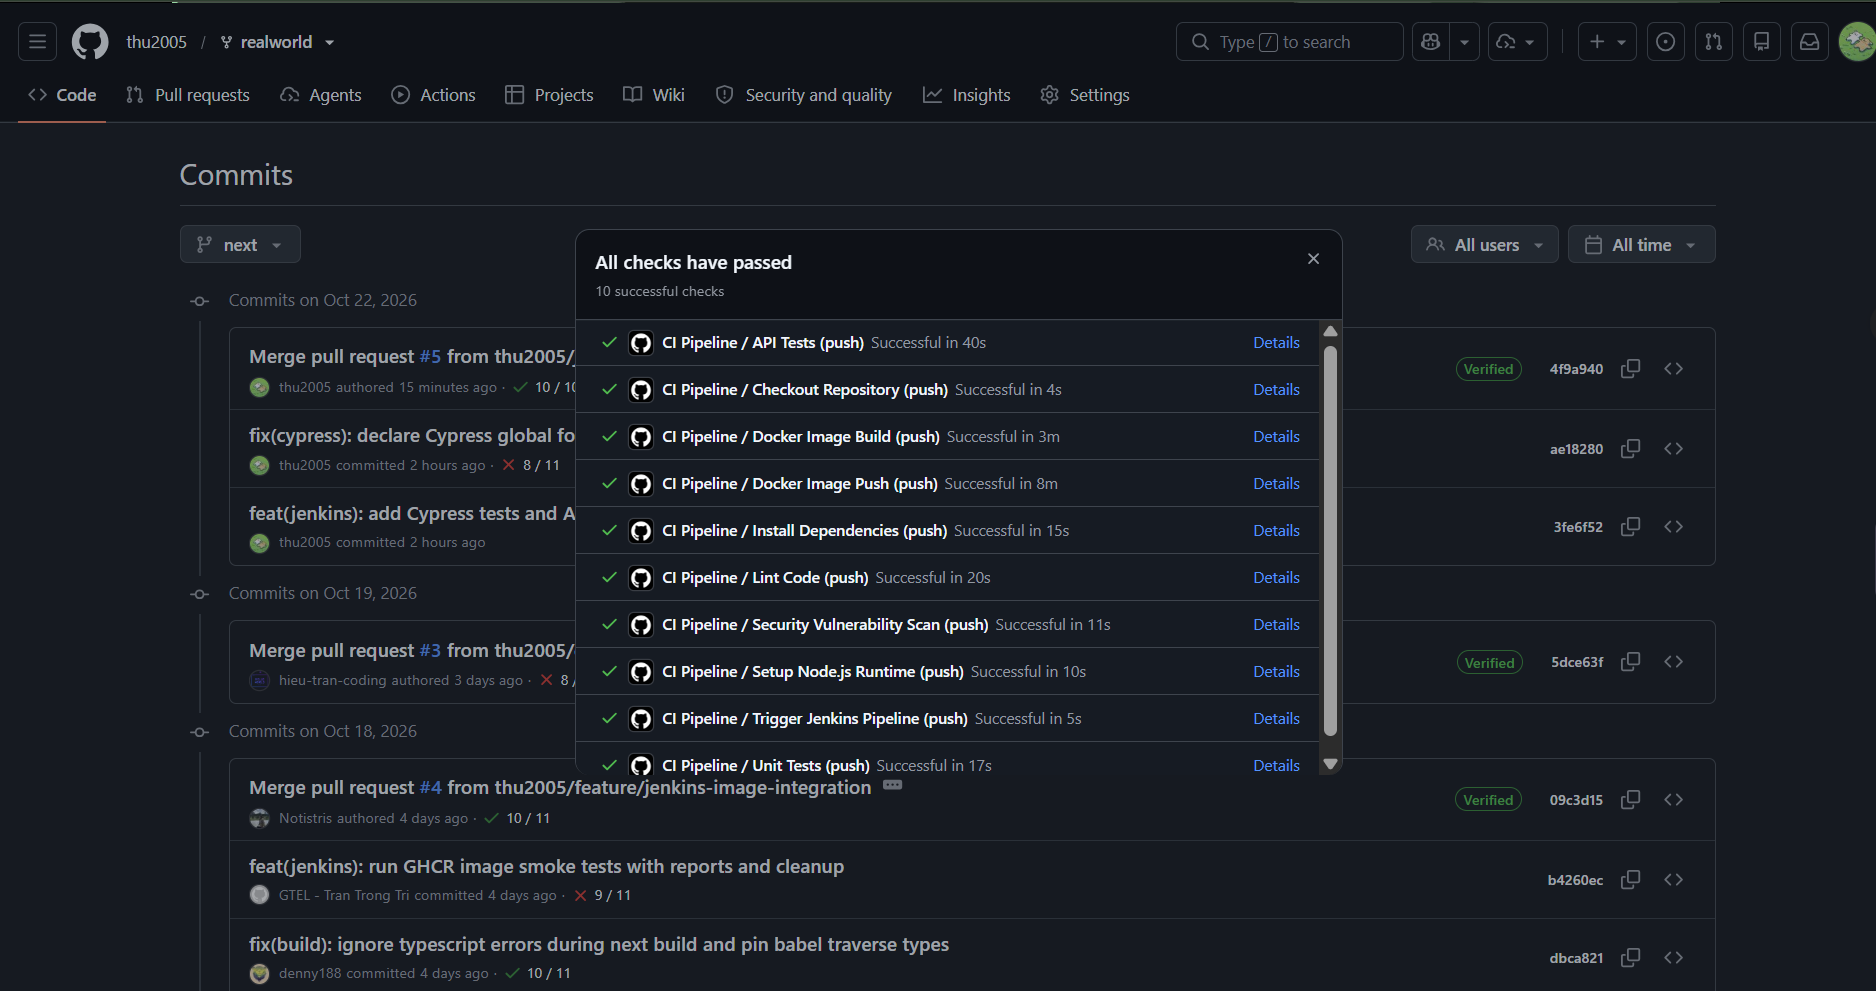
\includegraphics[keepaspectratio,alt={Mười checks của GitHub Actions thành công trên nhánh next}]{../weekly-docs/Week6/PersonD/screenshots/01-github-actions-next-all-checks-passed.png}}
\caption{Mười checks của GitHub Actions thành công trên nhánh next}
\end{figure}

\section{8.3. Kết quả kiểm tra phần hiện thực GitHub Actions mở
rộng}\label{83-kux1ebft-quux1ea3-kiux1ec3m-tra-phux1ea7n-hiux1ec7n-thux1ef1c-github-actions-mux1edf-rux1ed9ng}

Qua kiểm tra workflow tại revision \texttt{19c70a9}, pipeline chính có
11 job và workflow CodeQL có một job phân tích riêng. Các thay đổi có
thể đối chiếu trực tiếp trong cấu hình như sau:

\begin{longtable}[]{@{}
  >{\raggedright\arraybackslash}p{(\linewidth - 4\tabcolsep) * \real{0.2000}}
  >{\raggedright\arraybackslash}p{(\linewidth - 4\tabcolsep) * \real{0.4000}}
  >{\raggedright\arraybackslash}p{(\linewidth - 4\tabcolsep) * \real{0.4000}}@{}}
\toprule\noalign{}
\begin{minipage}[b]{\linewidth}\raggedright
Nội dung
\end{minipage} & \begin{minipage}[b]{\linewidth}\raggedright
Dấu hiệu trong mã nguồn
\end{minipage} & \begin{minipage}[b]{\linewidth}\raggedright
Kết quả mong đợi khi chạy
\end{minipage} \\
\midrule\noalign{}
\endhead
\bottomrule\noalign{}
\endlastfoot
JUnit cho Jest & Reporter \texttt{jest-junit}; \texttt{jest-unit.xml},
\texttt{jest-api.xml} & GitHub/Jenkins có thể đọc kết quả unit và API
theo cùng định dạng \\
Coverage artifact & \texttt{text}, \texttt{lcov}, \texttt{json-summary}
& Có báo cáo HTML, JSON summary và bảng trong Job Summary \\
Dependency security gate & \texttt{npm\ audit\ -\/-audit-level=high} &
Pipeline dừng khi phát hiện mức High/Critical \\
CodeQL SAST & \texttt{codeql.yml}, query
\texttt{security-extended,security-and-quality} & Kết quả được gửi đến
GitHub Code Scanning \\
Allure trên GitHub Actions & Job \texttt{allure-report}, artifact
\texttt{allure-report-dashboard} & Có báo cáo HTML tải từ workflow
run \\
\end{longtable}

\section{8.4. Kết quả unit test và
coverage}\label{84-kux1ebft-quux1ea3-unit-test-vuxe0-coverage}

GitHub Actions ghi nhận 3/3 Jest suites pass. Bảng coverage cho hai
mô-đun mục tiêu đạt 100\% statements, functions và lines; branch
coverage đạt 94,73\%, vượt threshold 80\%.

\begin{figure}
\centering
\pandocbounded{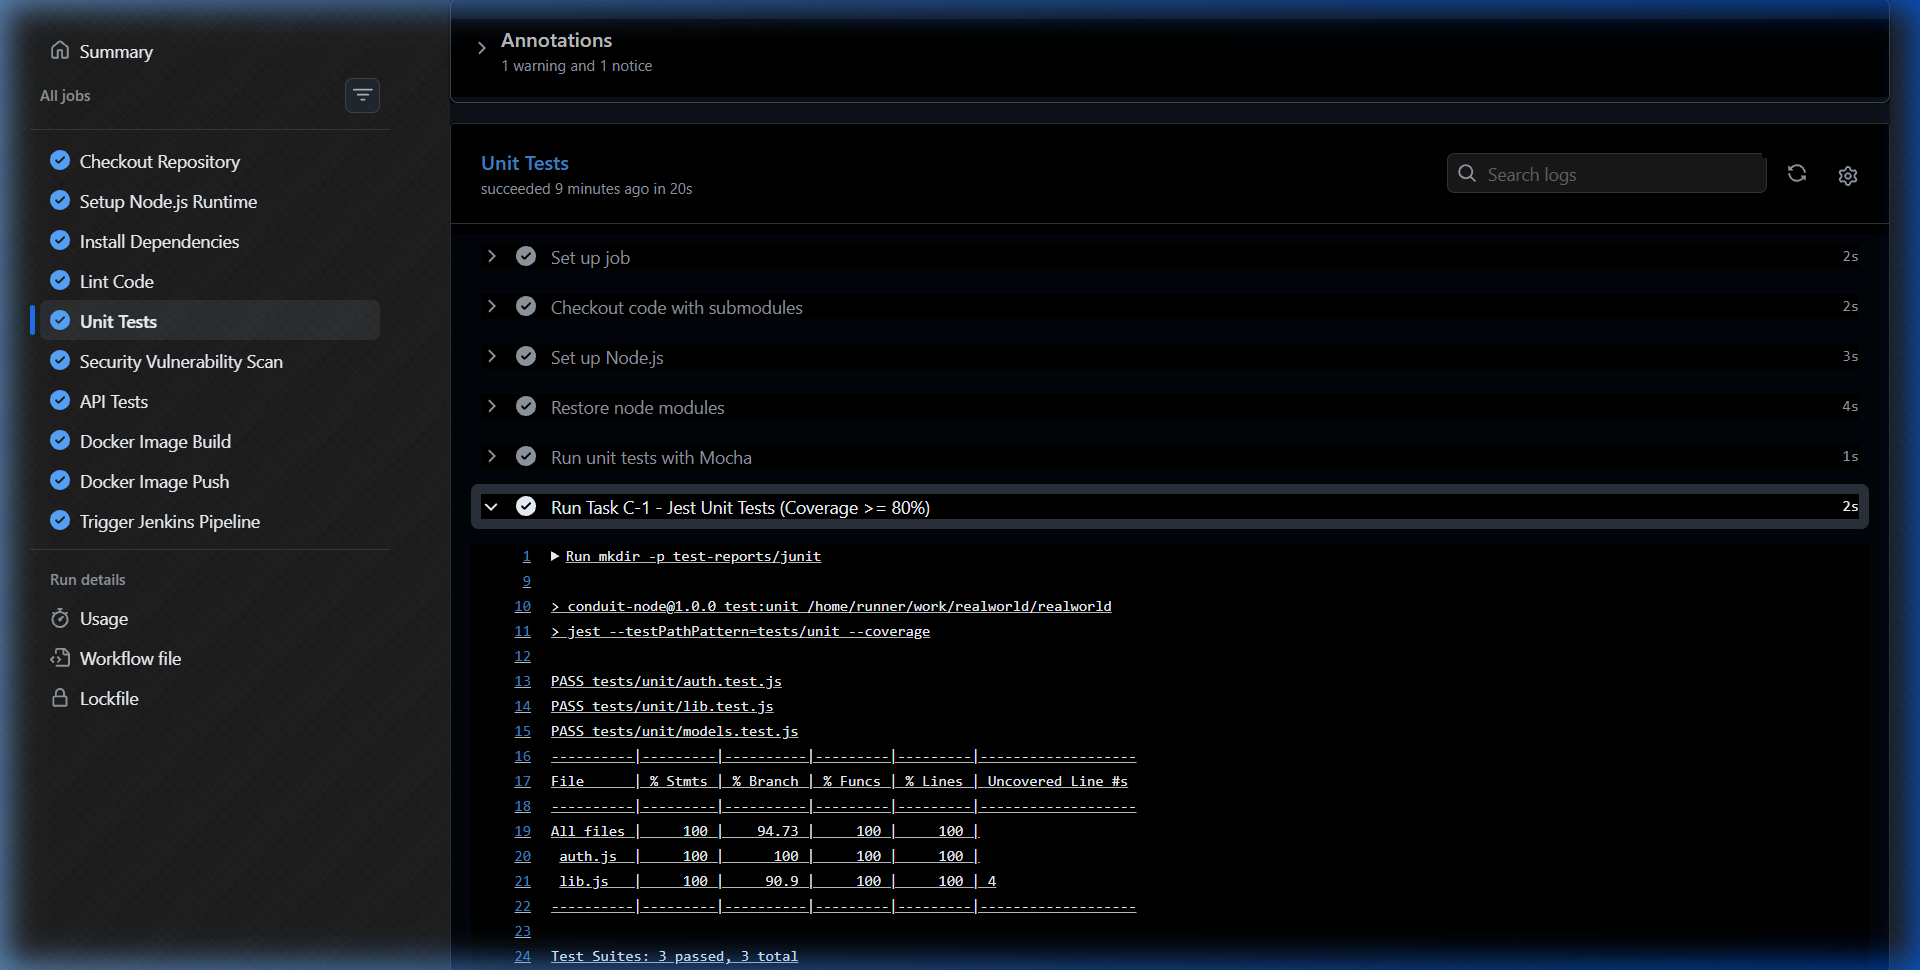
\includegraphics[keepaspectratio,alt={Unit test và coverage trong GitHub Actions}]{../weekly-docs/Week6/PersonC/screenshots/unit-tests-coverage-step.png}}
\caption{Unit test và coverage trong GitHub Actions}
\end{figure}

\section{8.5. Kết quả Jenkins image
pipeline}\label{85-kux1ebft-quux1ea3-jenkins-image-pipeline}

Jenkins Stage View cho thấy các bước prepare, validate, pull image, run
image, smoke test, kết nối UI runner và Cypress UI tests đều thành công.
Test Result Trend của build mới hơn hiển thị 6 kết quả pass, gồm 1 smoke
test và 5 Cypress tests. Artifact list chứa JUnit, Allure raw data,
video, log và integration summary.

\begin{figure}
\centering
\pandocbounded{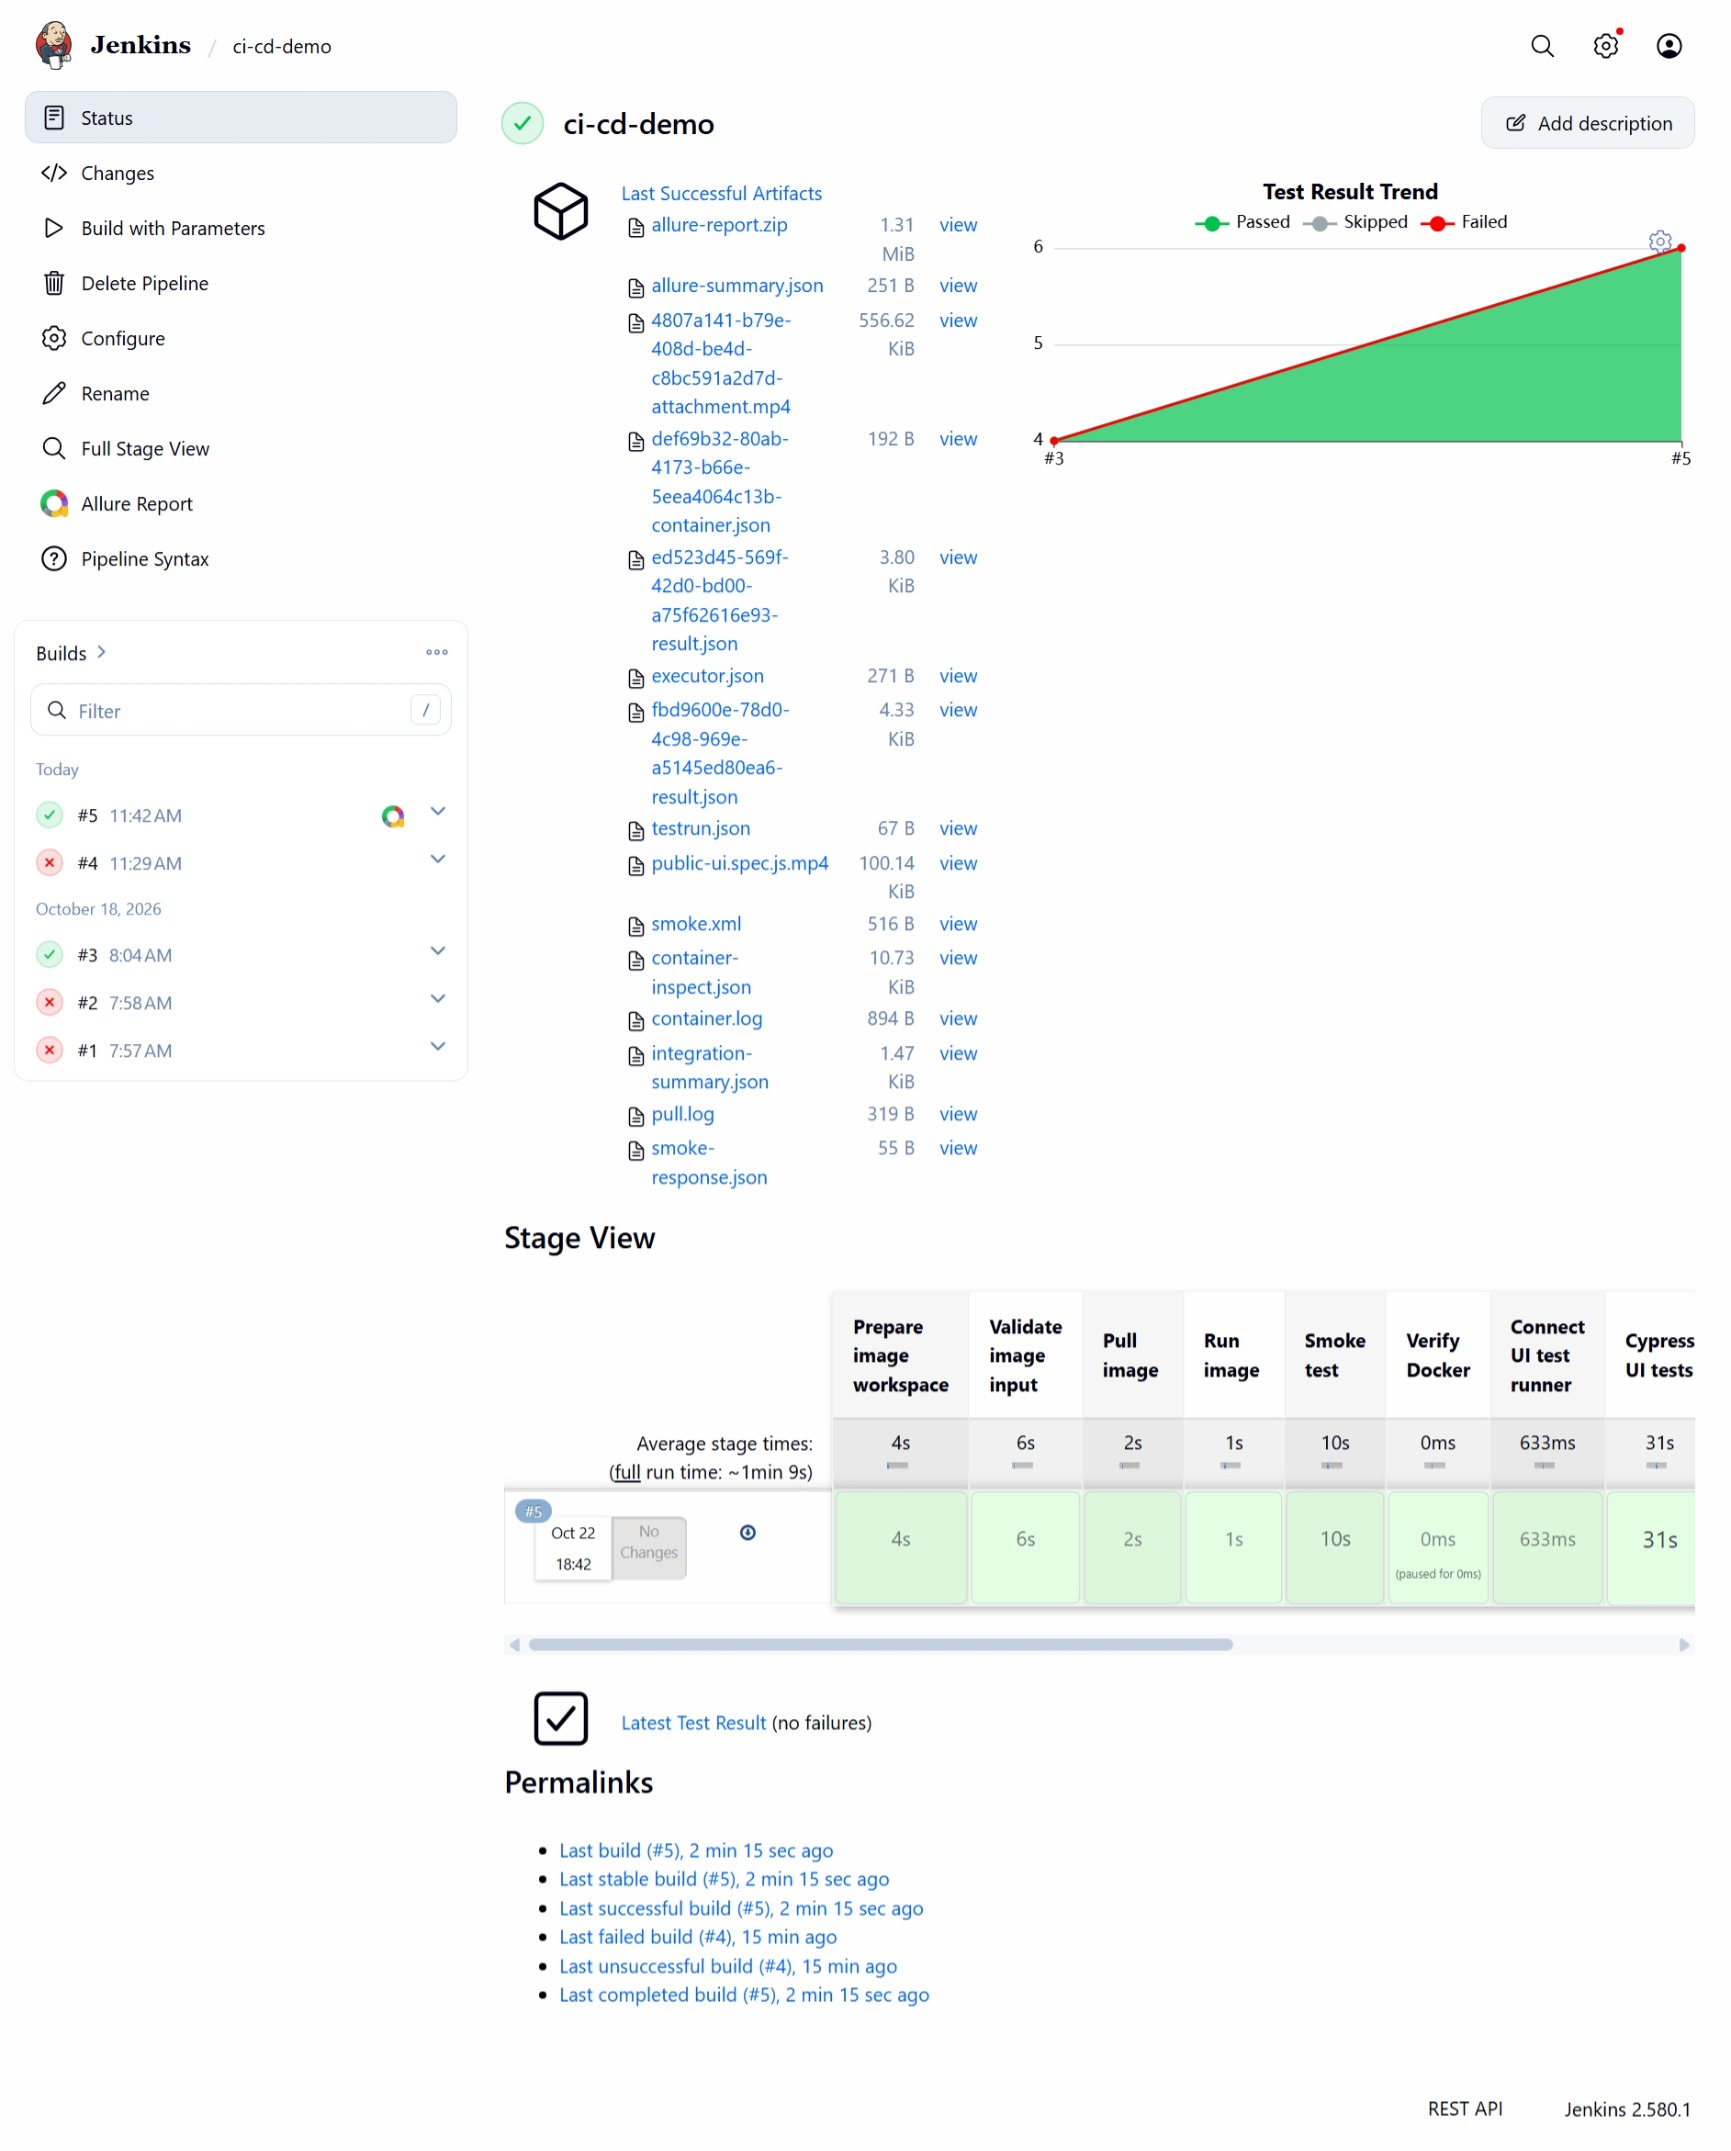
\includegraphics[keepaspectratio,alt={Jenkins image pipeline, test trend và artifacts}]{../weekly-docs/Week6/PersonD/screenshots/02-jenkins-cypress-stage-view-success.jpeg}}
\caption{Jenkins image pipeline, test trend và artifacts}
\end{figure}

Một lần kiểm chứng tích hợp Allure trước khi suite được mở rộng đã công
bố thành công 2/2 ca của \texttt{RealWorld\ public\ UI}. Bằng chứng này
xác nhận đường truyền dữ liệu Cypress → Allure raw results → Jenkins
Allure plugin hoạt động đúng.

\begin{figure}
\centering
\pandocbounded{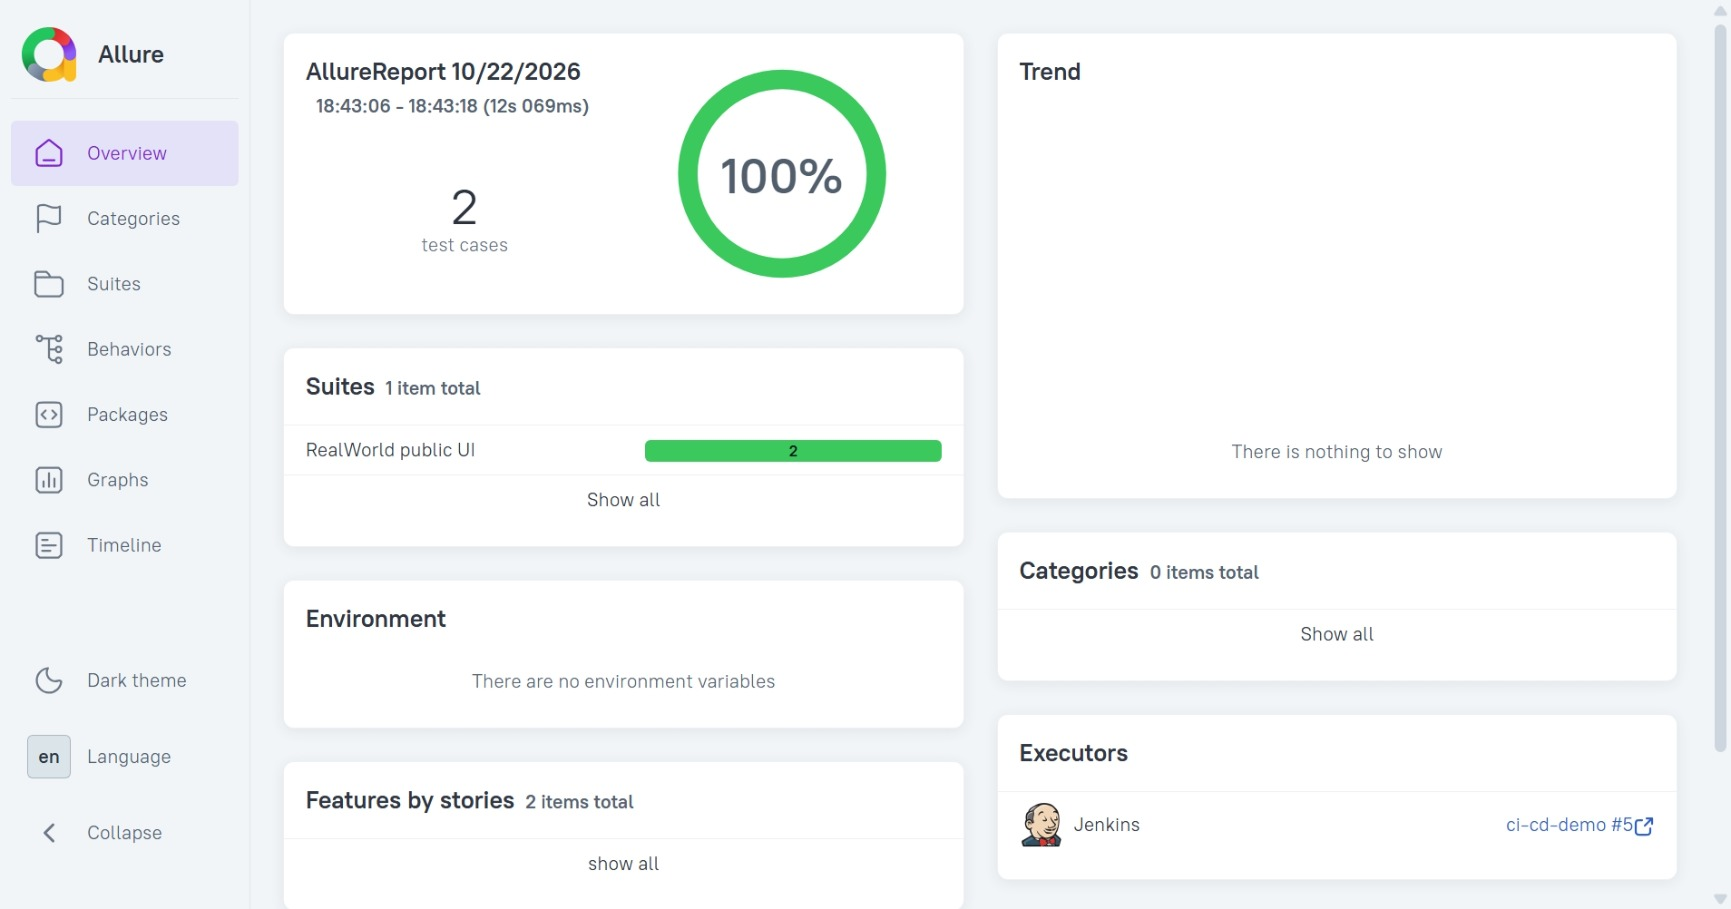
\includegraphics[keepaspectratio,alt={Allure Report được công bố từ Jenkins}]{../weekly-docs/Week6/PersonD/screenshots/03-allure-report-2-tests-passed.jpeg}}
\caption{Allure Report được công bố từ Jenkins}
\end{figure}

Build \texttt{\#9} kiểm chứng secure pull với
\texttt{GHCR\_PRIVATE=true}, revision \texttt{4f9a9405…}, test không lỗi
và danh sách artifact đầy đủ. Token không xuất hiện trên trang build.

\begin{figure}
\centering
\pandocbounded{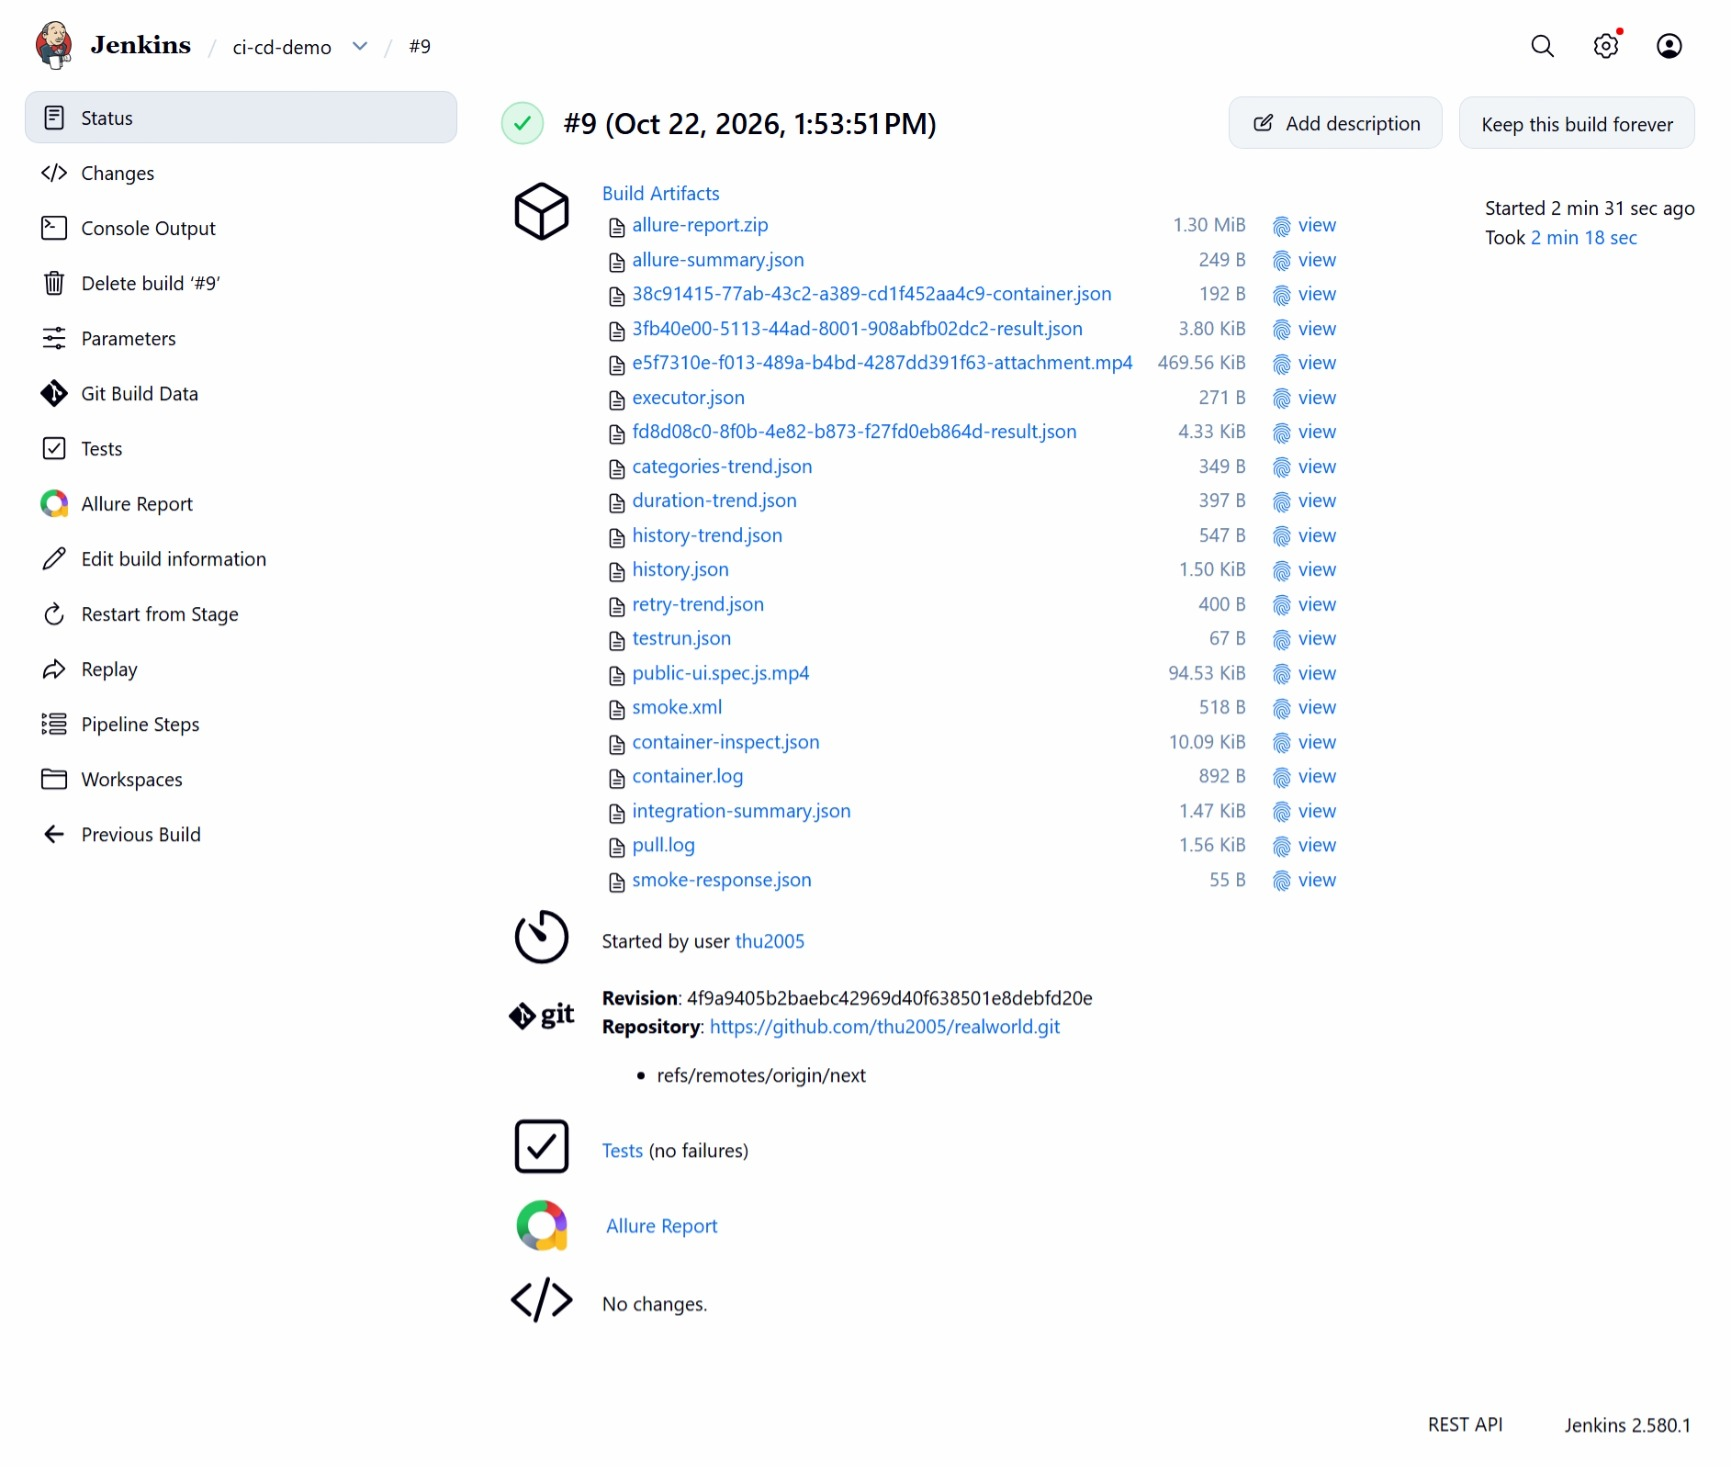
\includegraphics[keepaspectratio,alt={Jenkins build thành công với revision và artifacts có thể truy vết}]{../weekly-docs/Week6/PersonD/screenshots/04-jenkins-next-build-9-success.jpeg}}
\caption{Jenkins build thành công với revision và artifacts có thể truy
vết}
\end{figure}

\section{8.6. Tổng hợp kết
quả}\label{86-tux1ed5ng-hux1ee3p-kux1ebft-quux1ea3}

\begin{longtable}[]{@{}
  >{\raggedright\arraybackslash}p{(\linewidth - 4\tabcolsep) * \real{0.2400}}
  >{\raggedright\arraybackslash}p{(\linewidth - 4\tabcolsep) * \real{0.3200}}
  >{\raggedright\arraybackslash}p{(\linewidth - 4\tabcolsep) * \real{0.4400}}@{}}
\toprule\noalign{}
\begin{minipage}[b]{\linewidth}\raggedright
Hạng mục
\end{minipage} & \begin{minipage}[b]{\linewidth}\raggedright
Kết quả quan sát
\end{minipage} & \begin{minipage}[b]{\linewidth}\raggedright
Đánh giá
\end{minipage} \\
\midrule\noalign{}
\endhead
\bottomrule\noalign{}
\endlastfoot
GitHub Actions nền tảng & 10 checks thành công trên lần chạy có bằng
chứng & Đạt \\
GitHub Actions mở rộng & Cấu hình 11 job, JUnit, coverage summary và
Allure artifact & Đã hiện thực \\
Dependency security gate & Chặn mức High/Critical bằng
\texttt{npm\ audit\ -\/-audit-level=high} & Đã hiện thực \\
CodeQL SAST & Workflow JavaScript/TypeScript với bộ truy vấn mở rộng &
Đã hiện thực \\
Jest unit tests & 31 tests, 3 suites pass & Đạt \\
Coverage mục tiêu & 100/94,73/100/100, threshold 80\% & Đạt \\
SuperTest API & 15 test cases được tích hợp vào CI & Đạt \\
Docker build/smoke & Image build và \texttt{/api/tags} pass & Đạt \\
GHCR traceability & Image tag là full Git SHA & Đạt \\
Jenkins image lifecycle & Pull, run, smoke, Cypress và cleanup pass &
Đạt \\
Cypress hiện tại & 5 UI tests; Jenkins trend ghi 6 kết quả gồm smoke &
Đạt \\
Allure publication & Jenkins công bố report thành công & Đạt \\
Secret handling & Credential lấy qua Jenkins/GitHub secret store &
Đạt \\
\end{longtable}

\chapter{9. THẢO LUẬN}\label{9-thux1ea3o-luux1eadn}

\section{9.1. Ý nghĩa của kết
quả}\label{91-uxfd-nghux129a-cux1ee7a-kux1ebft-quux1ea3}

Kết quả quan trọng nhất không chỉ là số test pass mà là khả năng liên
kết các pha thành một chuỗi có thể kiểm chứng. Một Git commit tạo ra một
image mang cùng SHA; Jenkins dùng chính SHA này để kéo image; build lưu
report và log gắn với lần chạy. Chuỗi liên kết đó làm cho câu hỏi ``đã
kiểm tra phiên bản nào?'' có câu trả lời rõ ràng.

Việc giữ source mode song song với image mode cũng có giá trị chẩn đoán.
Source mode cho biết repository có thể lint, test và build trong
Jenkins. Image mode cho biết artifact do CI tạo có thể vận hành. Nếu
source mode pass nhưng image mode fail, phạm vi điều tra có thể tập
trung vào Dockerfile, registry hoặc runtime container.

\section{9.2. Vai trò của test harness trong giải
pháp}\label{92-vai-truxf2-cux1ee7a-test-harness-trong-giux1ea3i-phuxe1p}

Nếu chỉ có các file test, người dùng vẫn phải tự khởi động server, chọn
port, chờ readiness, chạy đúng lệnh và thu report. Harness đã biến các
thao tác này thành quy trình xác định: nó tạo môi trường, điều phối
container, cung cấp base URL cho Cypress, thu bằng chứng và dọn tài
nguyên. Đây là khác biệt thực tế giữa một tập test scripts và một test
harness tích hợp.

\section{9.3. Đánh đổi thiết
kế}\label{93-ux111uxe1nh-ux111ux1ed5i-thiux1ebft-kux1ebf}

Chạy Cypress bên trong custom Jenkins image giúp cấu hình demo đơn giản
và report xuất hiện trực tiếp ở Jenkins, nhưng làm Jenkins image lớn
hơn. Gắn Docker socket giúp quản lý sibling container thuận tiện, song
chỉ an toàn khi Jenkins chạy job đáng tin cậy. Việc dùng hai nền tảng CI
tăng giá trị minh họa về handoff và artifact verification, đồng thời làm
cấu hình phức tạp hơn một pipeline đơn lẻ.

Nhóm ưu tiên khả năng tái hiện và truy vết hơn việc tối ưu thời gian
chạy tuyệt đối. Ví dụ, tag SHA được dùng làm định danh chính dù vẫn có
tag \texttt{latest} phụ trợ; full SHA dài hơn nhưng không mơ hồ.

\chapter{10. KHÓ KHĂN, GIỚI HẠN VÀ HƯỚNG PHÁT
TRIỂN}\label{10-khuxf3-khux103n-giux1edbi-hux1ea1n-vuxe0-hux1b0ux1edbng-phuxe1t-triux1ec3n}

\section{10.1. Khó khăn trong quá trình thực
hiện}\label{101-khuxf3-khux103n-trong-quuxe1-truxecnh-thux1ef1c-hiux1ec7n}

Ứng dụng dùng Node.js 14 và nhiều dependency cũ, trong khi runner và
plugin hiện đại thường giả định runtime mới hơn. Nhóm phải cố định
Node/npm và chọn phiên bản Cypress tương thích. Repository không commit
lockfile nên việc cài dependency chưa có tính tất định hoàn toàn.

Jenkins chạy trên máy local tại \texttt{127.0.0.1:18080}; GitHub-hosted
runner không thể truy cập địa chỉ localhost này. Vì vậy, khả năng tự
động trigger đã được hiện thực ở mức client và contract, nhưng các lần
kiểm chứng local sử dụng \textbf{Build with Parameters} sau khi image
được push. Việc đưa Jenkins ra Internet chỉ để demo sẽ tạo rủi ro lớn
hơn lợi ích.

Quá trình tích hợp qua nhiều nhánh làm bằng chứng được tạo ở các mốc
khác nhau. Ảnh Allure xác nhận 2 test ban đầu, trong khi source hiện tại
đã mở rộng lên 5 Cypress tests và Jenkins Test Trend ghi nhận 5 UI tests
cộng 1 smoke test. Báo cáo phân biệt rõ hai mốc thay vì dùng ảnh cũ để
suy diễn kết quả mới.

\section{10.2. Giới hạn}\label{102-giux1edbi-hux1ea1n}

\begin{itemize}
\tightlist
\item
  Coverage mới được thu thập có chủ đích cho \texttt{lib.js} và
  \texttt{auth.js}, chưa đại diện toàn bộ ứng dụng.
\item
  UI suite tập trung vào public navigation và validation, chưa bao phủ
  toàn bộ luồng người dùng đã xác thực.
\item
  Cổng \texttt{npm\ audit} chặn lỗ hổng mức High/Critical, nhưng cây
  dependency cũ có thể làm pipeline dừng cho đến khi nhóm nâng cấp hoặc
  thay thế các gói liên quan.
\item
  Phần Allure trên GitHub Actions đã có cấu hình tạo artifact, nhưng báo
  cáo thực nghiệm hiện có chủ yếu chứng minh Allure trên Jenkins.
\item
  Jenkins chạy test trên controller để đơn giản hóa seminar; mô hình vận
  hành thực tế nên dùng agent cô lập.
\item
  Kết nối GitHub Actions → Jenkins chưa được chứng minh qua một địa chỉ
  Jenkins có thể truy cập từ Internet hoặc self-hosted runner trong lần
  demo local.
\end{itemize}

\section{10.3. Hướng phát
triển}\label{103-hux1b0ux1edbng-phuxe1t-triux1ec3n}

Hệ thống có thể được hoàn thiện theo thứ tự ưu tiên sau:

\begin{enumerate}
\def\labelenumi{\arabic{enumi}.}
\tightlist
\item
  Commit lockfile và nâng cấp runtime/dependency trong một nhánh riêng
  để tăng tính lặp lại và giảm lỗ hổng.
\item
  Mở rộng coverage có chọn lọc sang route và model quan trọng, đồng thời
  giữ threshold phù hợp với phạm vi đo.
\item
  Bổ sung UI tests cho đăng nhập thành công, tạo bài viết, bình luận và
  đăng xuất bằng dữ liệu kiểm thử cô lập.
\item
  Dùng self-hosted runner hoặc một địa chỉ Jenkins được bảo vệ để kiểm
  chứng quá trình kích hoạt tự động từ đầu đến cuối mà không công khai
  tùy tiện máy local.
\item
  Chuyển Jenkins workload sang agent tạm thời, giới hạn quyền Docker và
  tách controller khỏi test execution.
\item
  Duy trì việc xử lý cảnh báo từ \texttt{npm\ audit} và CodeQL, đồng
  thời bổ sung bằng chứng thực nghiệm cho Allure artifact trên GitHub
  Actions.
\end{enumerate}

\chapter{11. VIDEO DEMO}\label{11-video-demo}

Ba video của seminar được tổ chức theo ba nội dung độc lập. Liên kết sẽ
được điền vào bản Markdown sau khi nhóm xuất bản video và trước khi tạo
PDF chính thức.

\begin{longtable}[]{@{}
  >{\raggedleft\arraybackslash}p{(\linewidth - 4\tabcolsep) * \real{0.2400}}
  >{\raggedright\arraybackslash}p{(\linewidth - 4\tabcolsep) * \real{0.3200}}
  >{\raggedright\arraybackslash}p{(\linewidth - 4\tabcolsep) * \real{0.4400}}@{}}
\toprule\noalign{}
\begin{minipage}[b]{\linewidth}\raggedleft
Video
\end{minipage} & \begin{minipage}[b]{\linewidth}\raggedright
Nội dung
\end{minipage} & \begin{minipage}[b]{\linewidth}\raggedright
Liên kết
\end{minipage} \\
\midrule\noalign{}
\endhead
\bottomrule\noalign{}
\endlastfoot
1 & Cơ sở lý thuyết và kiến trúc tổng thể của giải pháp & \emph{Chờ nhóm
cung cấp URL} \\
2 & GitHub Actions: pipeline 11 job, CodeQL, kiểm thử, Docker build và
GHCR push & \emph{Chờ nhóm cung cấp URL} \\
3 & Jenkins: image mode, smoke test, Cypress, Allure và cleanup &
\emph{Chờ nhóm cung cấp URL} \\
\end{longtable}

\chapter{12. KẾT LUẬN}\label{12-kux1ebft-luux1eadn}

Seminar đã hiện thực một test harness nhiều lớp cho RealWorld và tích
hợp nó vào hai nền tảng tự động hóa. GitHub Actions chịu trách nhiệm
kiểm tra source và tạo container artifact; Jenkins kiểm chứng artifact
đó bằng smoke test và UI tests, sau đó công bố report và dọn môi trường.
Các bộ Jest, SuperTest, Newman, Mocha và Cypress cung cấp phản hồi ở các
mức khác nhau; JUnit, Allure, log và video tạo bằng chứng để phân tích.

Qua quá trình thực hiện, nhóm nhận thấy giá trị của CI/CD không nằm ở số
lượng stage mà ở tính nhất quán của đầu vào, điều kiện pass/fail và
artifact đầu ra. Tương tự, test harness không chỉ là tập hợp test
scripts mà là toàn bộ cơ chế giúp test được thiết lập, thực thi, quan
sát và kết thúc có kiểm soát. Việc dùng full commit SHA, chuẩn hóa
report path và lưu kết quả hậu xử lý đã giúp các phân hệ do nhiều thành
viên phát triển có thể tích hợp thành một quy trình chung có khả năng
tái hiện.

\chapter{TÀI LIỆU THAM KHẢO}\label{tuxe0i-liux1ec7u-tham-khux1ea3o}

{[}1{]} ISTQB, \emph{Glossary of Testing Terms}, mục ``testing'',
\url{https://glossary.istqb.org/}.

{[}2{]} Martin Fowler, ``Continuous Integration,'' 2006,
\url{https://martinfowler.com/articles/continuousIntegration.html}.

{[}3{]} Jez Humble và David Farley, \emph{Continuous Delivery: Reliable
Software Releases through Build, Test, and Deployment Automation},
Addison-Wesley, 2010.

{[}4{]} Jenkins Project, ``Pipeline,'' \emph{Jenkins User
Documentation}, \url{https://www.jenkins.io/doc/book/pipeline/}.

{[}5{]} GitHub, ``Understanding GitHub Actions,'' \emph{GitHub Docs},
\url{https://docs.github.com/actions/about-github-actions/understanding-github-actions}.

{[}6{]} ISO/IEC/IEEE 24765:2017, \emph{Systems and software engineering
--- Vocabulary}, International Organization for Standardization, 2017.

{[}7{]} Mike Cohn, \emph{Succeeding with Agile: Software Development
Using Scrum}, Addison-Wesley, 2009.

{[}8{]} Jest, ``Jest Documentation,''
\url{https://jestjs.io/docs/getting-started}.

{[}9{]} SuperAgent contributors, ``SuperTest,''
\url{https://github.com/ladjs/supertest}.

{[}10{]} Postman, ``Newman Documentation,''
\url{https://learning.postman.com/docs/collections/using-newman-cli/command-line-integration-with-newman/}.

{[}11{]} Cypress, ``Cypress Documentation,''
\url{https://docs.cypress.io/}.

{[}12{]} Allure Report, ``Allure Report Documentation,''
\url{https://allurereport.org/docs/}.

{[}13{]} Docker, ``Docker Build Overview,''
\url{https://docs.docker.com/build/concepts/overview/}.

{[}14{]} GitHub, ``Working with the Container registry,''
\url{https://docs.github.com/packages/working-with-a-github-packages-registry/working-with-the-container-registry}.

\end{document}
